\documentclass{article}
\usepackage{fancyhdr}
\usepackage{setspace}
\usepackage{titlesec}
\usepackage{graphicx}
\usepackage{float}
\usepackage[style=apa, sorting=nyt]{biblatex}
\usepackage{geometry}
\usepackage{hyperref}

\geometry{a4paper, margin=1in}
% \addbibresource{references.bib}

\begin{document}

% ---------- Cover page ----------
\begin{titlepage}
\begin{center}
\vspace*{1cm}

Swinburne University of Technology \\
School of Science, Computing, and Emerging Technologies
\vspace{8cm}

SWE40006 - Software Deployment and Evolution \\
\textbf{Deployment Portfolio Task 1}
\vfill

Student name: Ngoc Van Nhi Do \\
Student ID: 105551765
\end{center}
\end{titlepage}

% ---------- Header + footer ----------
\pagestyle{fancy}
\fancyhead[L]{Ngoc Van Nhi Do}
\fancyhead[R]{105551765}
\fancyfoot{}
\renewcommand{\footrulewidth}{0.4pt}% default is 0pt
\fancyfoot[L]{SWE40006 - Software Deployment and Evolution (Semester 2 2026 - Due August 18, 2026)}
\fancyfoot[R]{\small\thepage}

\newpage

\begin{center}
\vspace*{2px}
{\LARGE
\setlength{\baselineskip}{2em}
Deployment Portfolio Task 1
}
\end{center}

\section{Declared Target Level}

All four subtasks 1.1, 1.2, 1.3, and 1.4 were attempted. The technologies used include Visual Studio 2022 (v.17.14.37), WiX v7, and the HeatWave extension installed on the IDE.

\section{Execution Evidence}
\subsection{Task 1.1}
I built and packaged a sample console application into an .msi installer using WiX 7.0.0 via the Command-line Interface (CLI).

The first step is creating a new C\# project, adding the provided code, and building it in Release mode.

\begin{figure}[H]
\centering
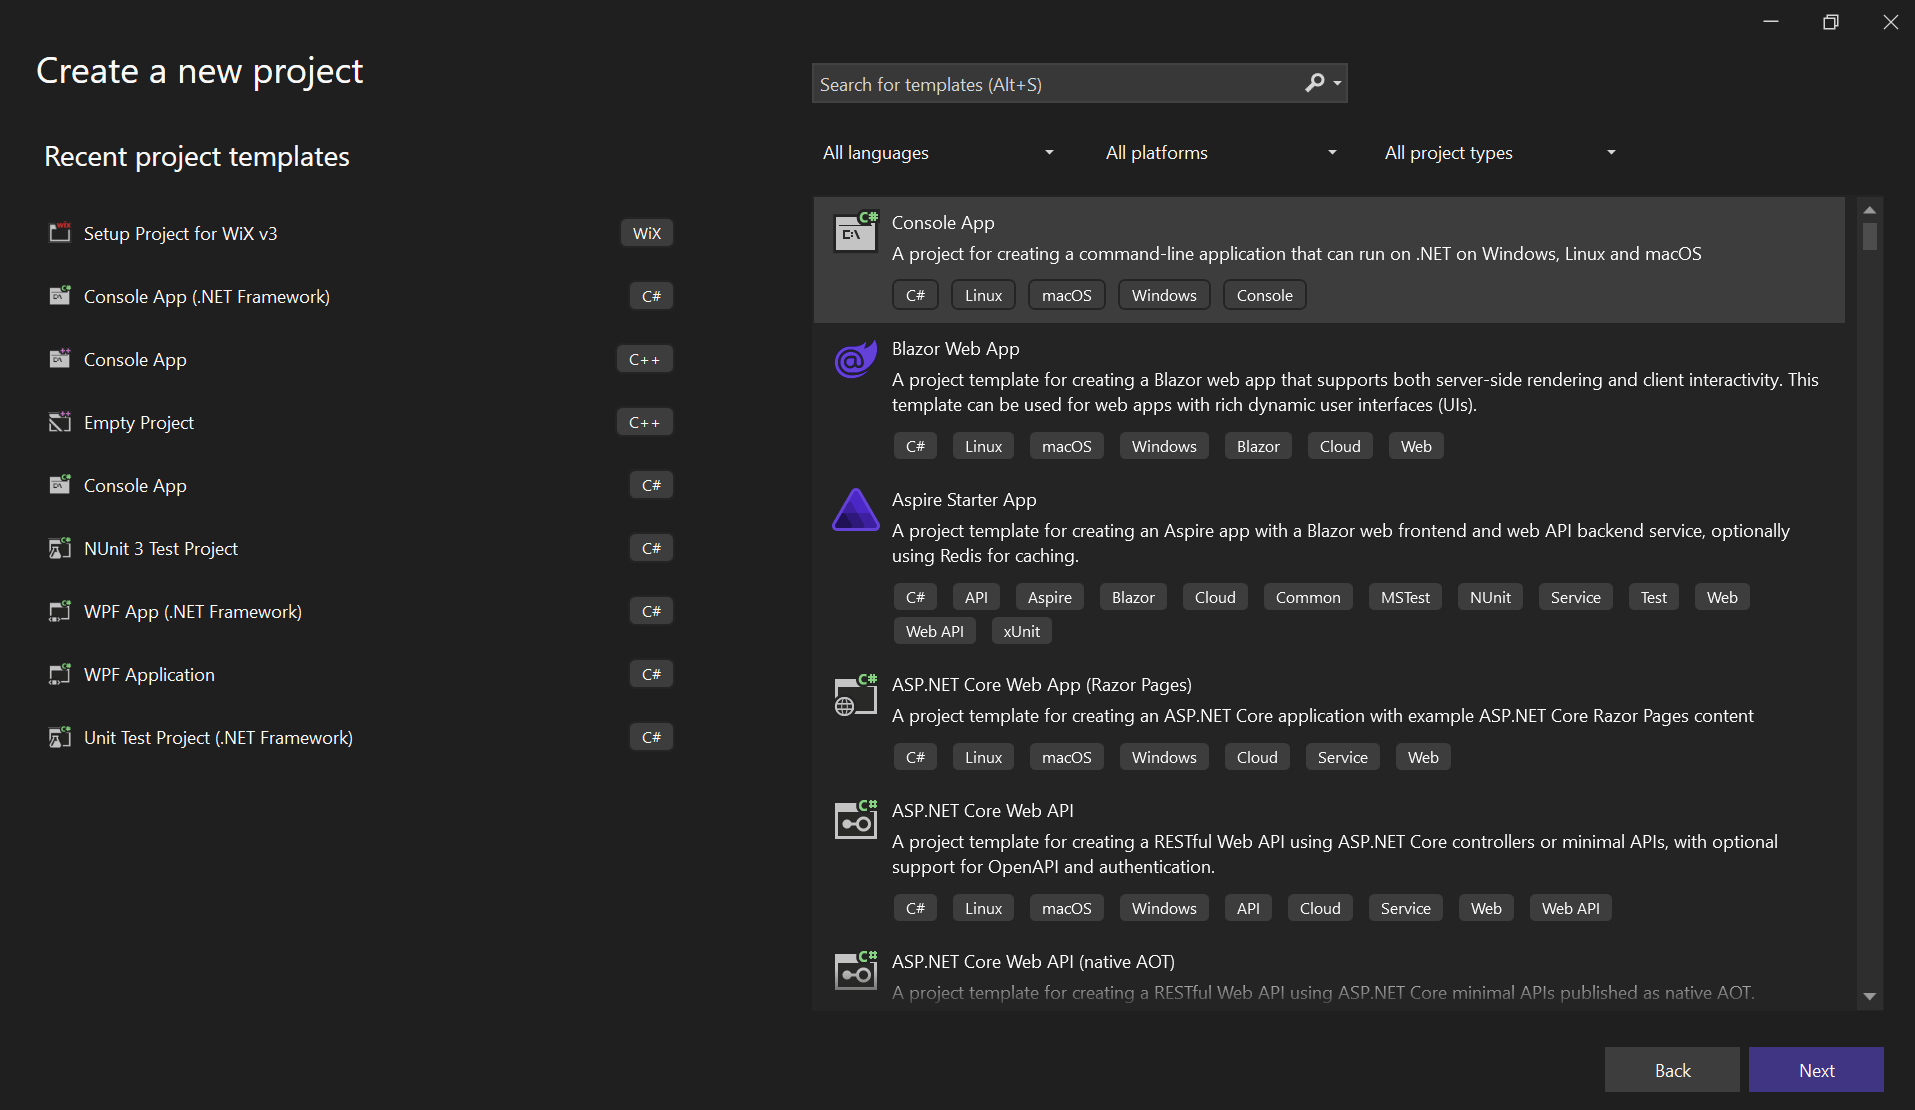
\includegraphics[scale=0.4]{images/1_create_project.jpg}
\vspace{-1em}
\caption{Creating a new C\# console application.}
\end{figure}

\begin{figure}[H]
\centering
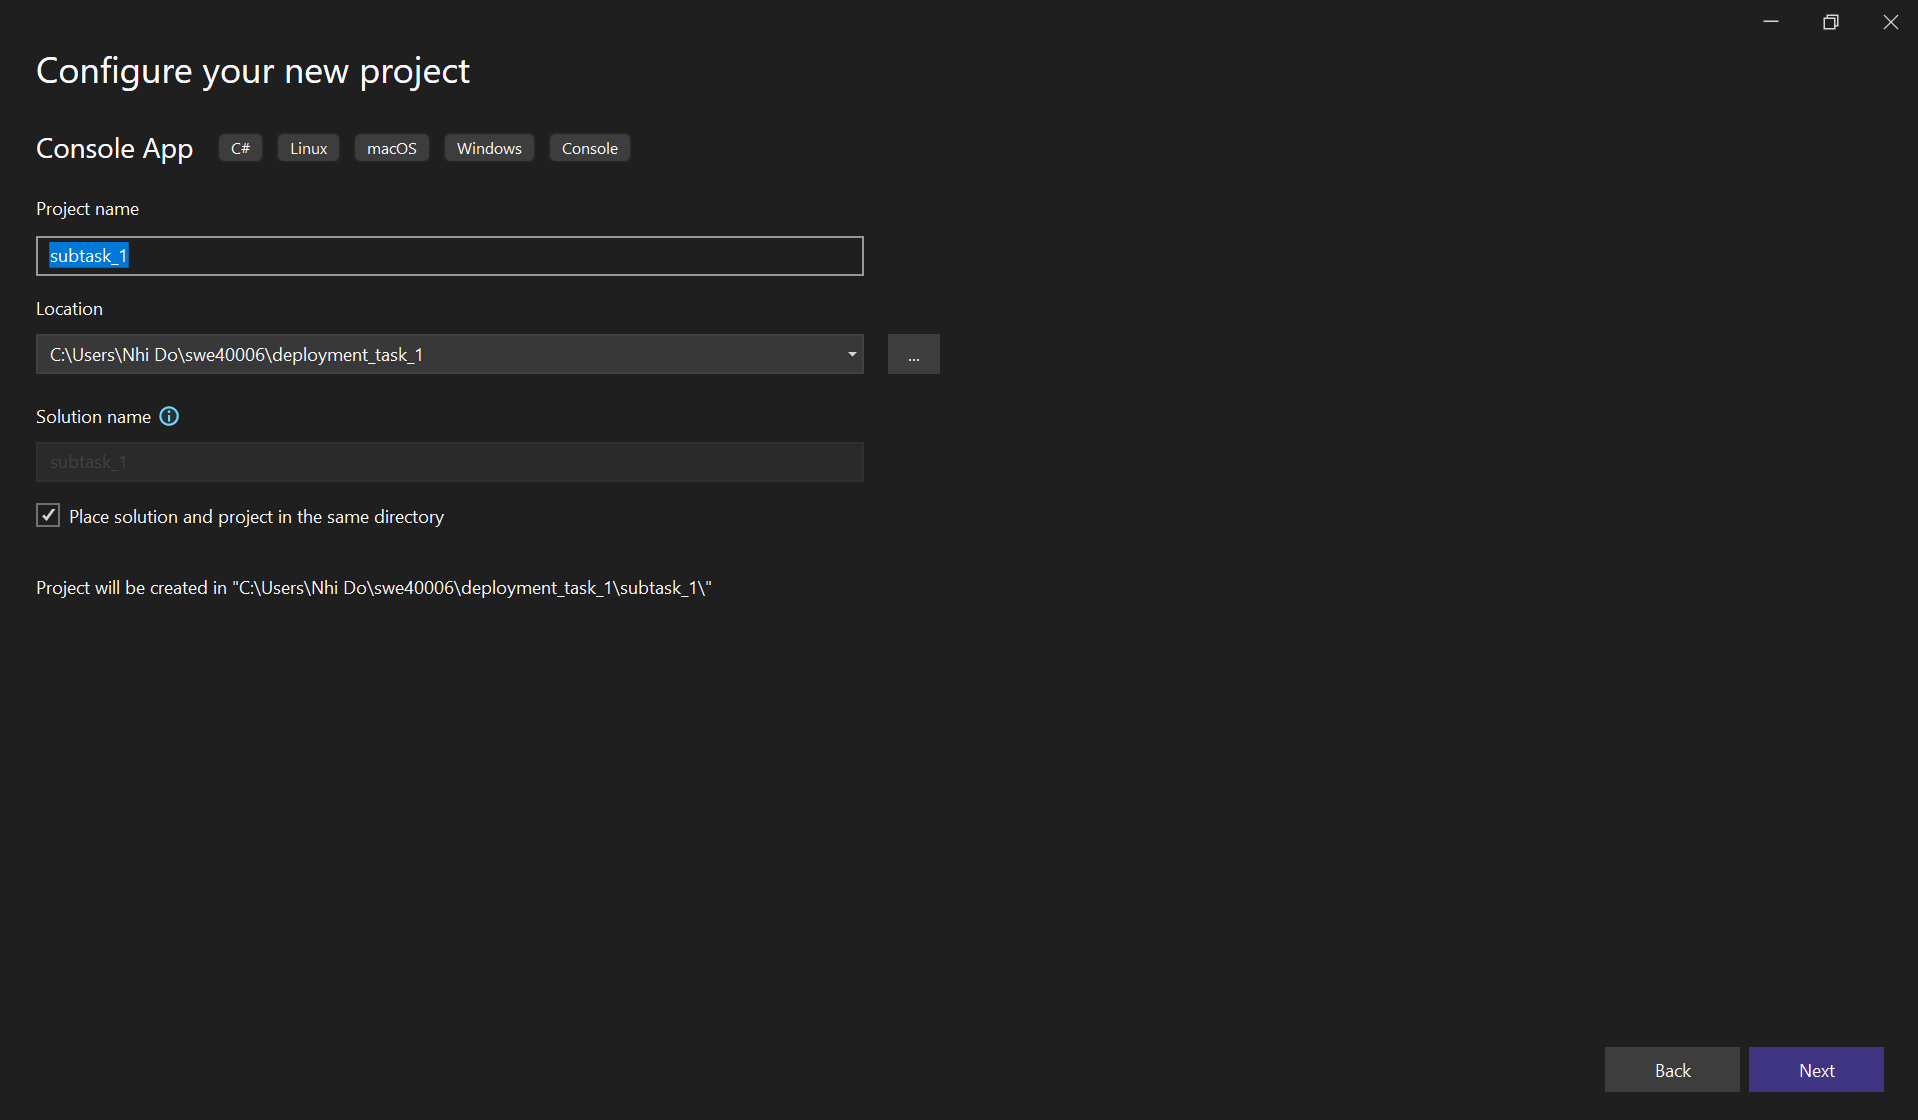
\includegraphics[scale=0.4]{images/1_name_project.jpg}
\vspace{-1em}
\caption{Naming the application.}
\end{figure}

\begin{figure}[H]
\centering
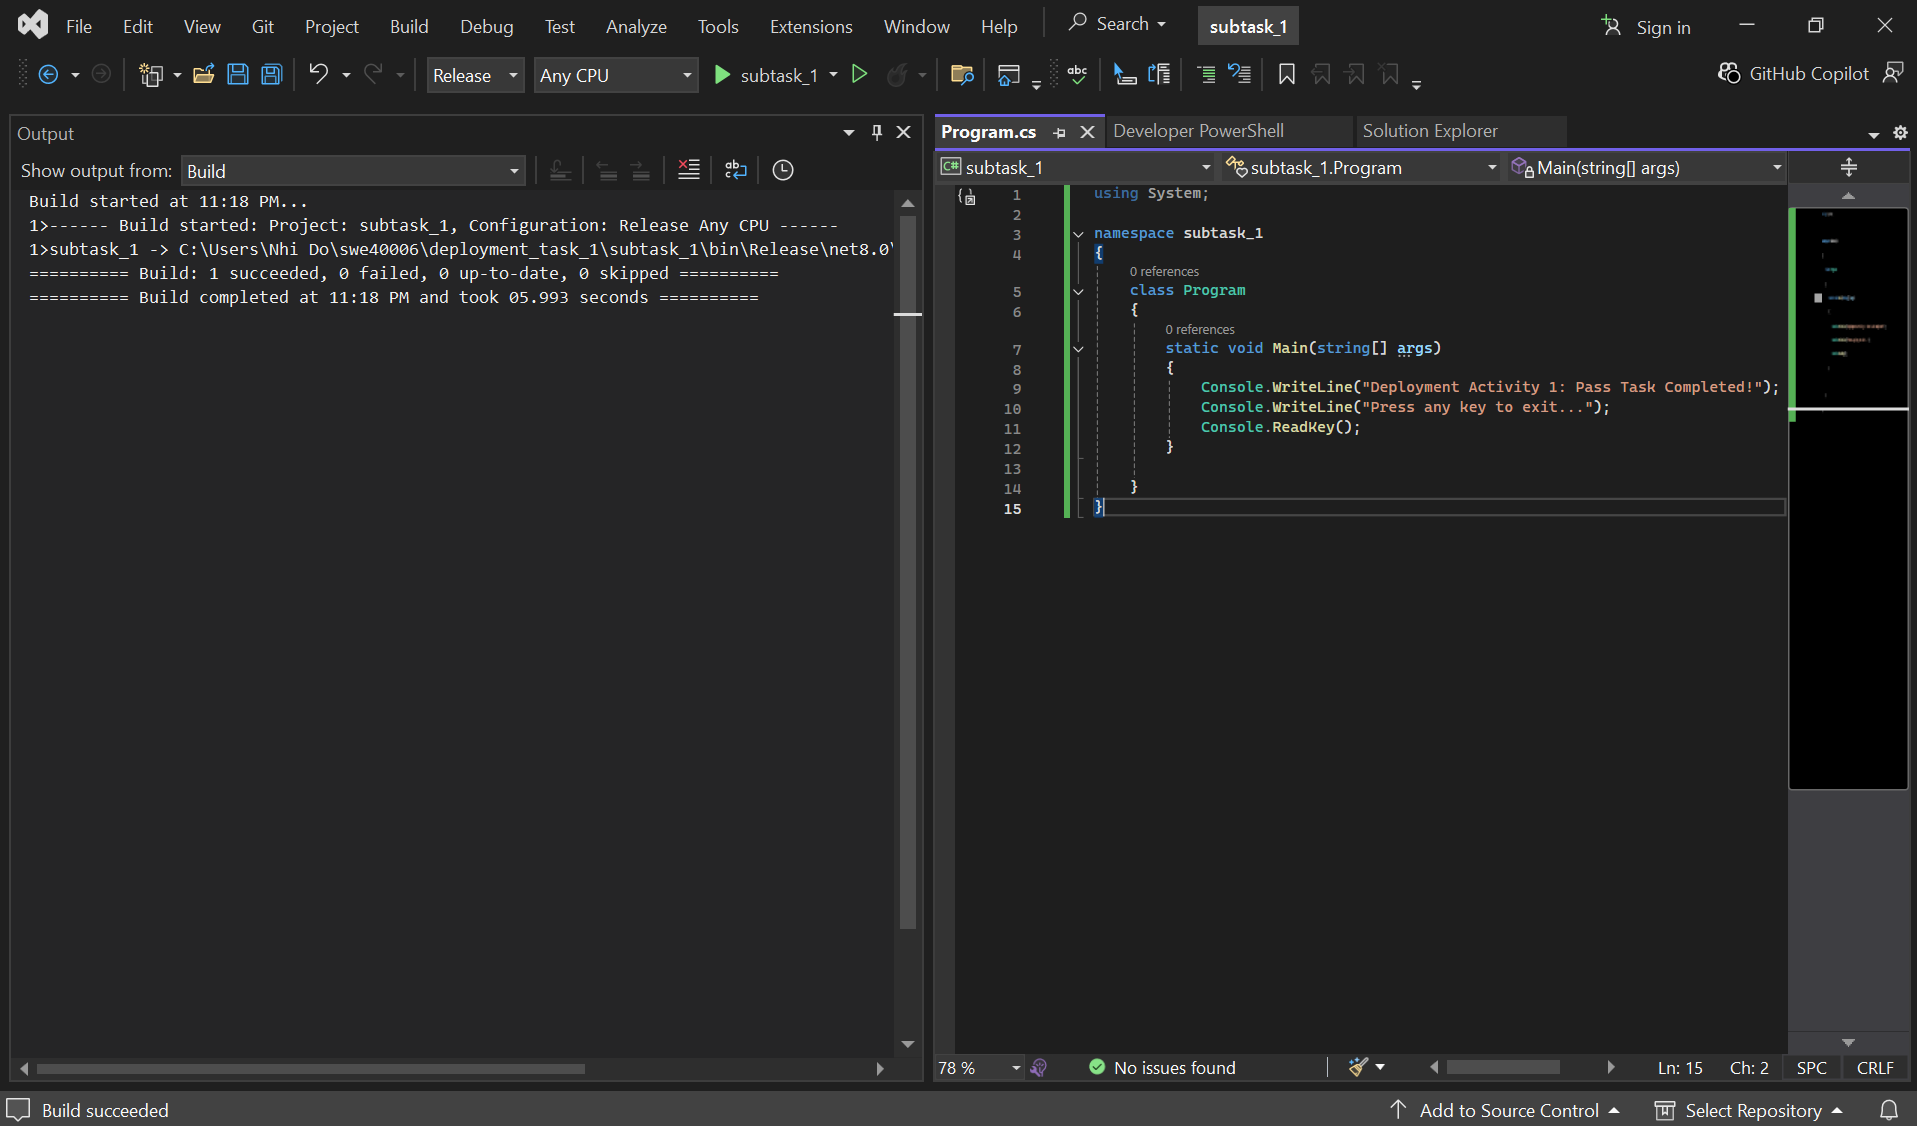
\includegraphics[scale=0.4]{images/1_build_project.jpg}
\vspace{-1em}
\caption{Building the program in Release mode.}
\end{figure}

Once the program has been built, its executable is created the project's \texttt{bin\\Release} folder.

The WiX toolset is installed using the CLI.

\begin{figure}[H]
\centering
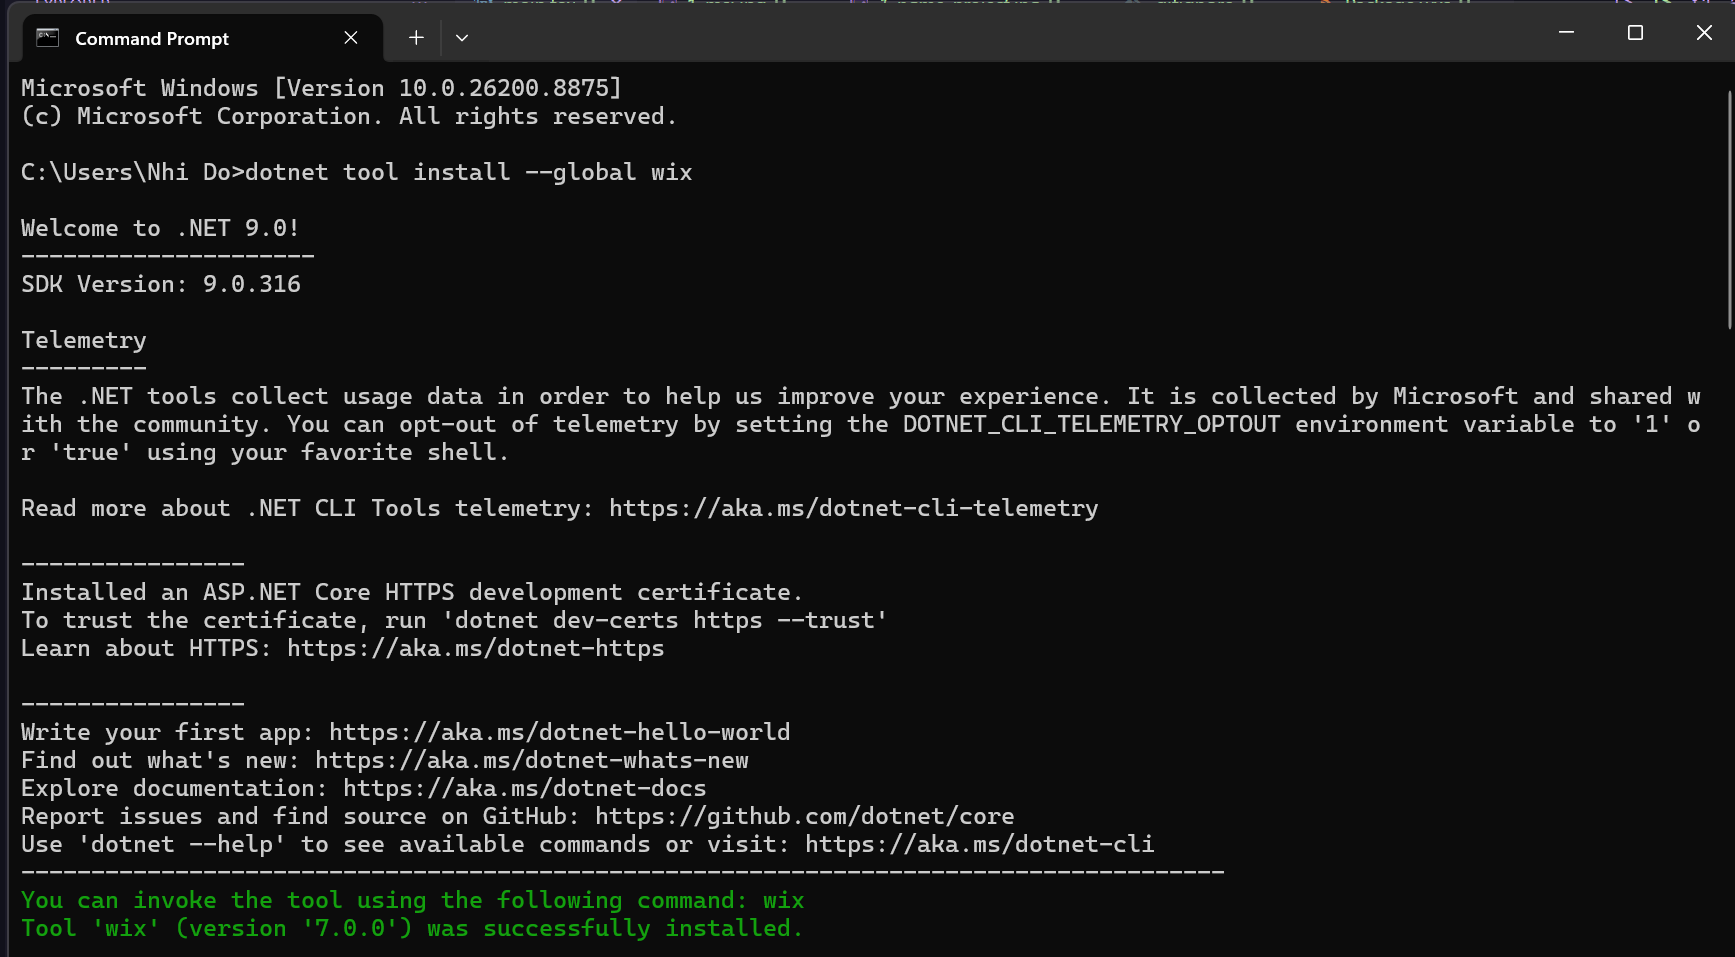
\includegraphics[scale=0.4]{images/1_install_wix.jpg}
\vspace{-1em}
\caption{Installing WiX.}
\end{figure}

The WiX project and source file are manually created. The \texttt{.wxs} file is then configured to contain instructions to build the installer. The file specifies the application name, manufacturer, version, and upgrade code, as well as the directory in which the application will be installed. It also defines the application files that should be included in the installer and groups them into the feature.

\begin{figure}[H]
\centering
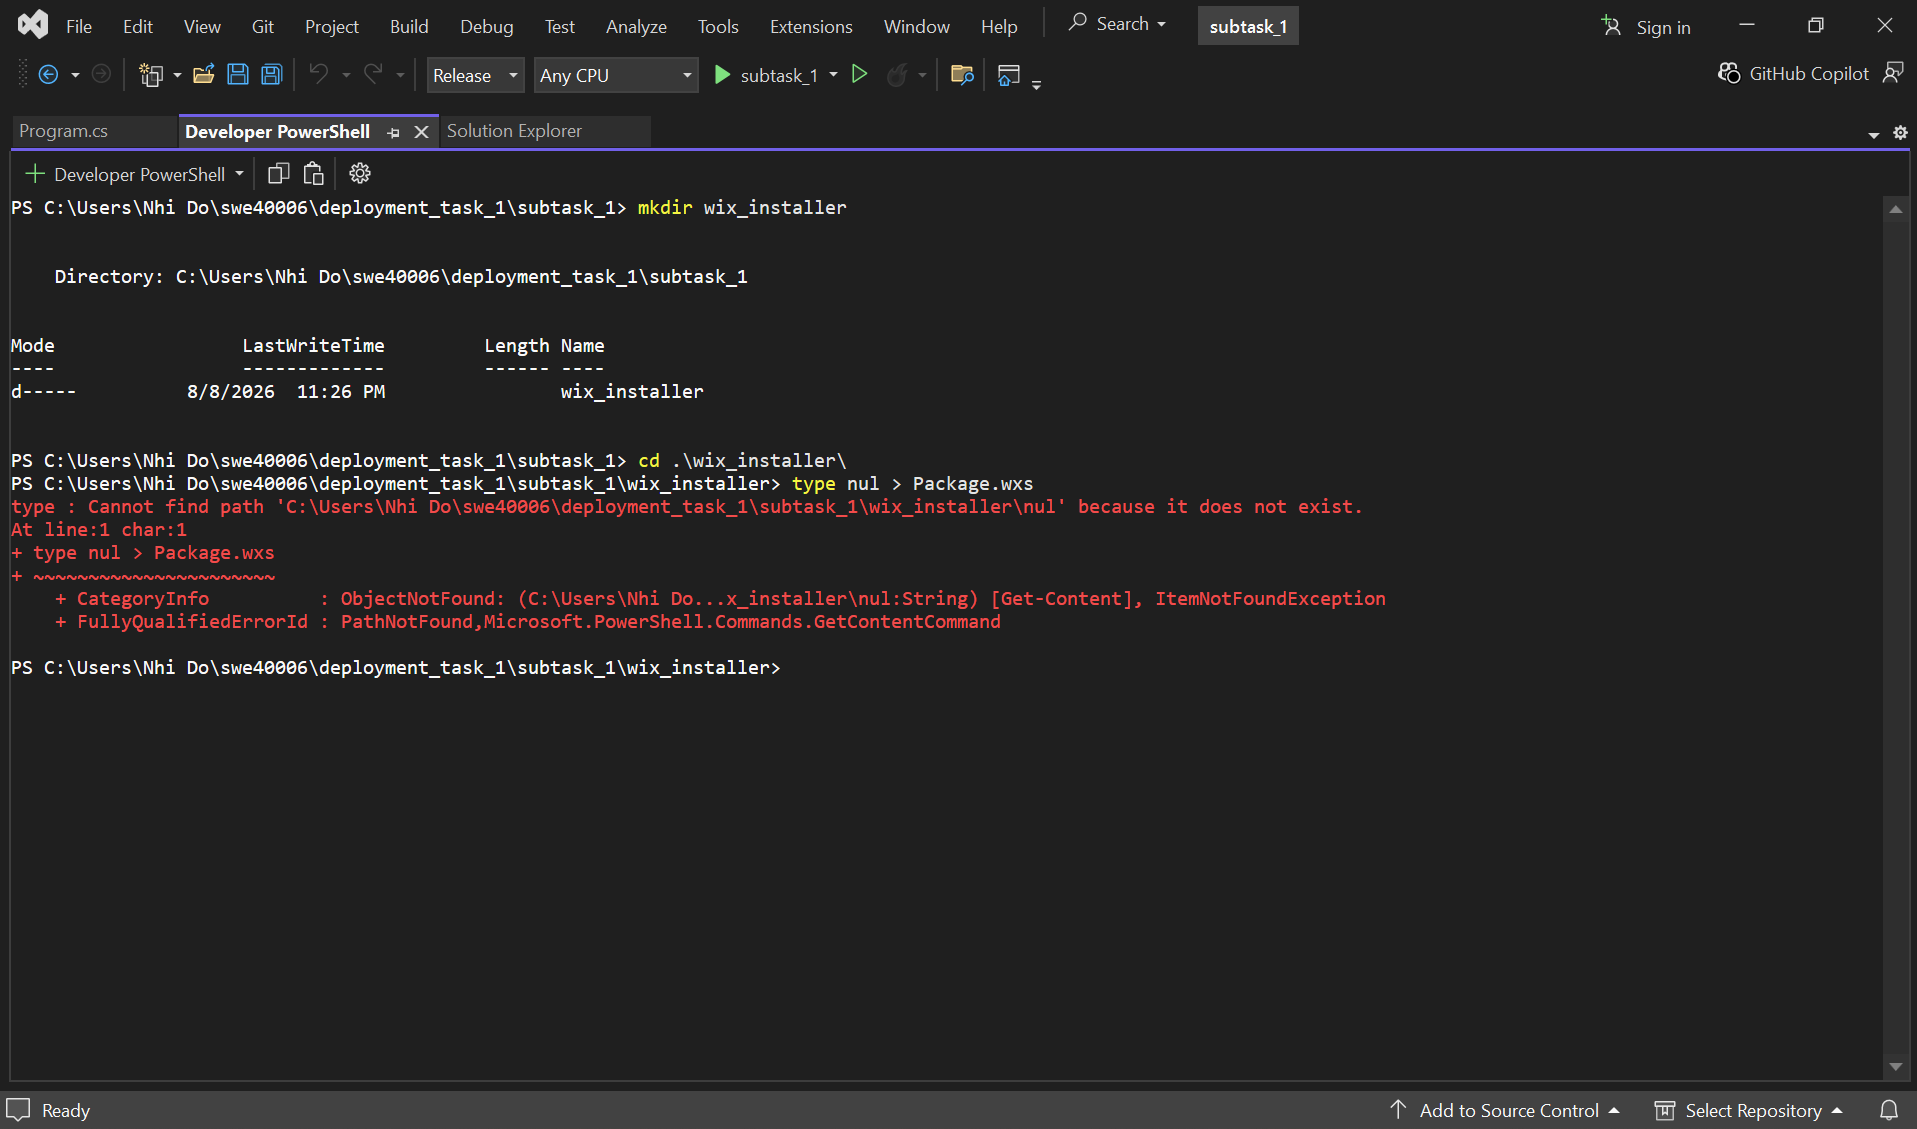
\includegraphics[scale=0.4]{images/1_create_wix.jpg}
\vspace{-1em}
\caption{Creating the WiX installer project and source file.}
\end{figure}

\begin{figure}[H]
\centering
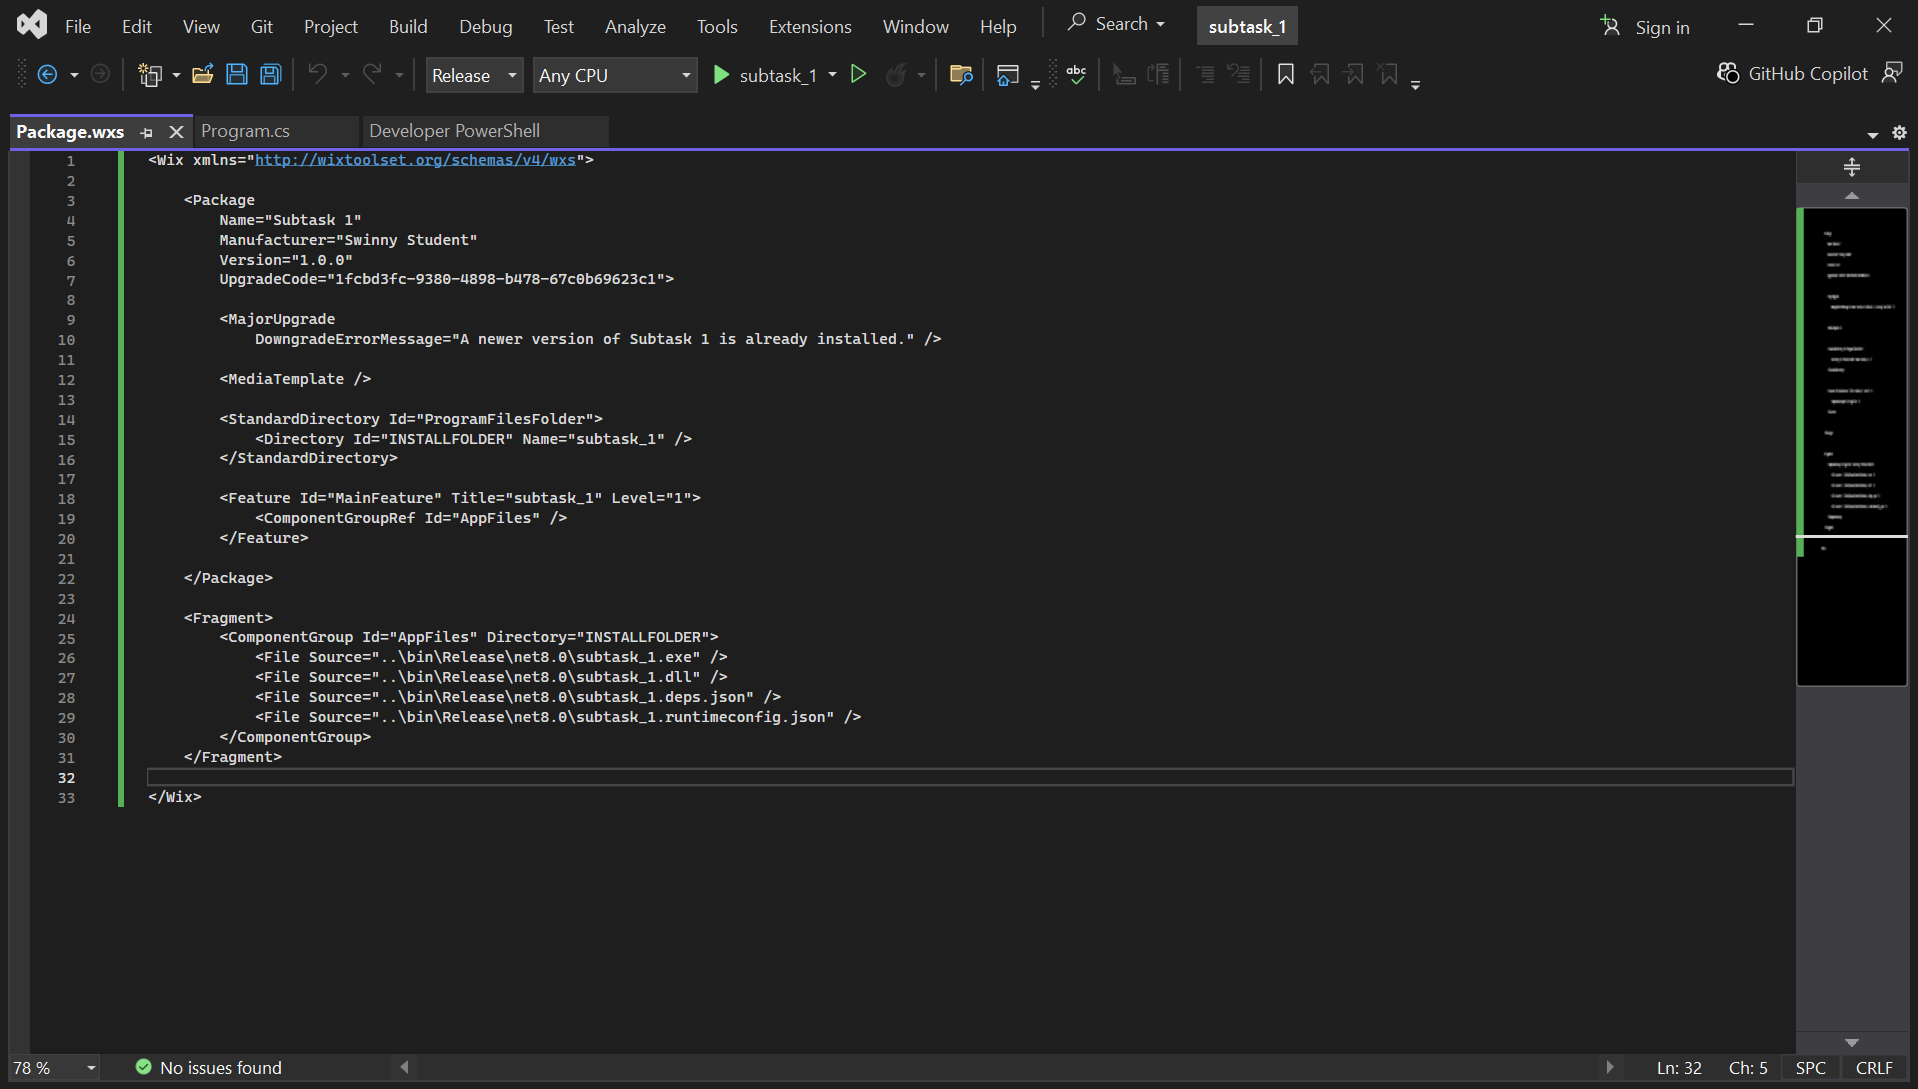
\includegraphics[scale=0.4]{images/1_create_wxs.jpg}
\vspace{-1em}
\caption{Configuring the Package.wxs file to build the installer.}
\end{figure}

The installer is then built using the command below. The resulting MSI file is created inside the installer directory.

\begin{figure}[H]
\centering
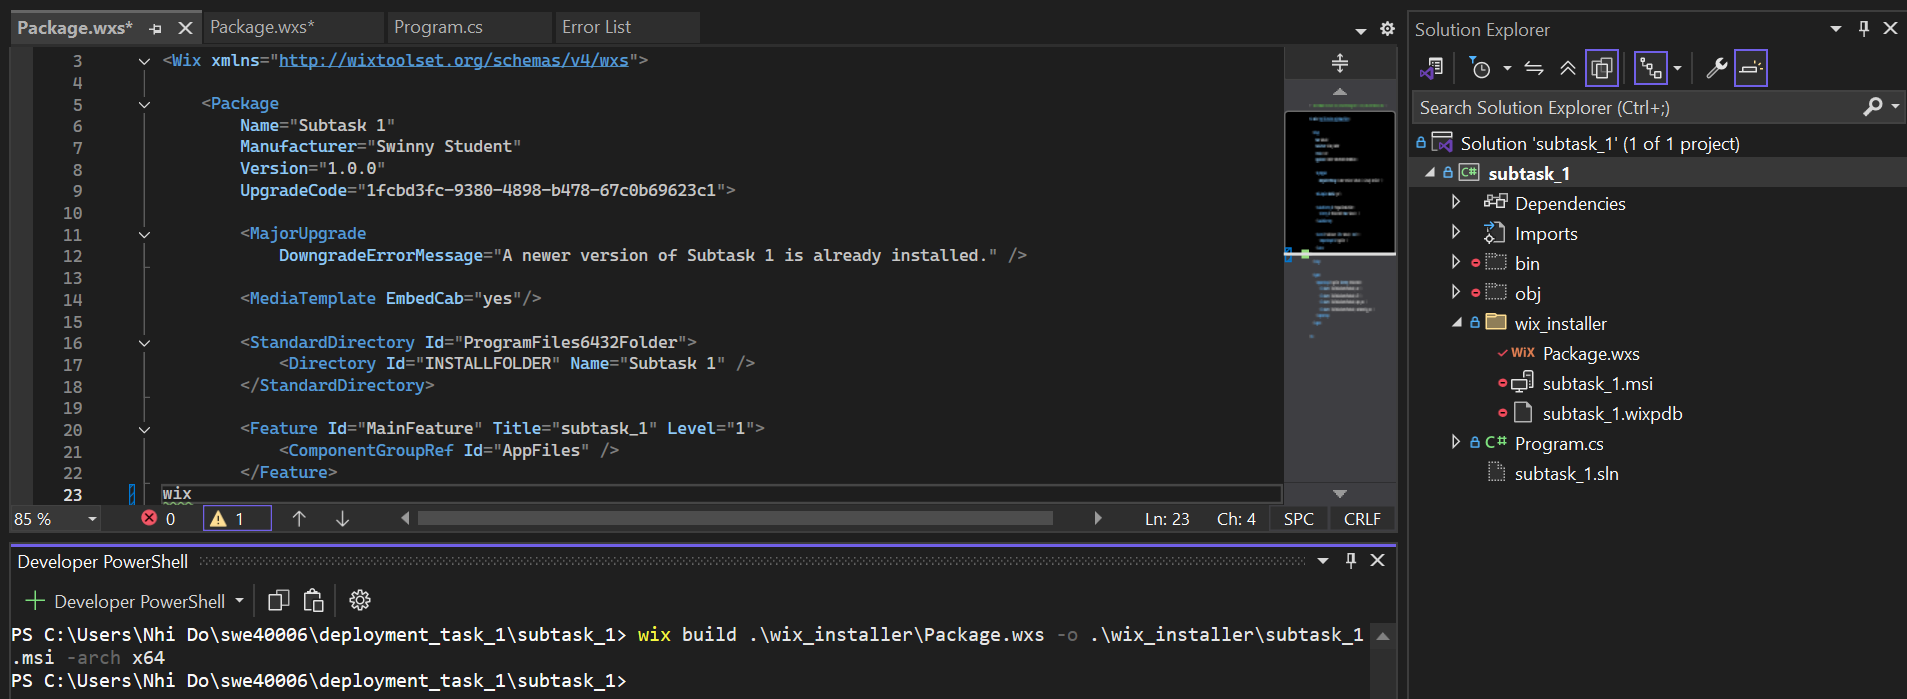
\includegraphics[scale=0.4]{images/1_build_msi.jpg}
\vspace{-1em}
\caption{Building the installer from the WiX source file.}
\end{figure}

\begin{figure}[H]
\centering
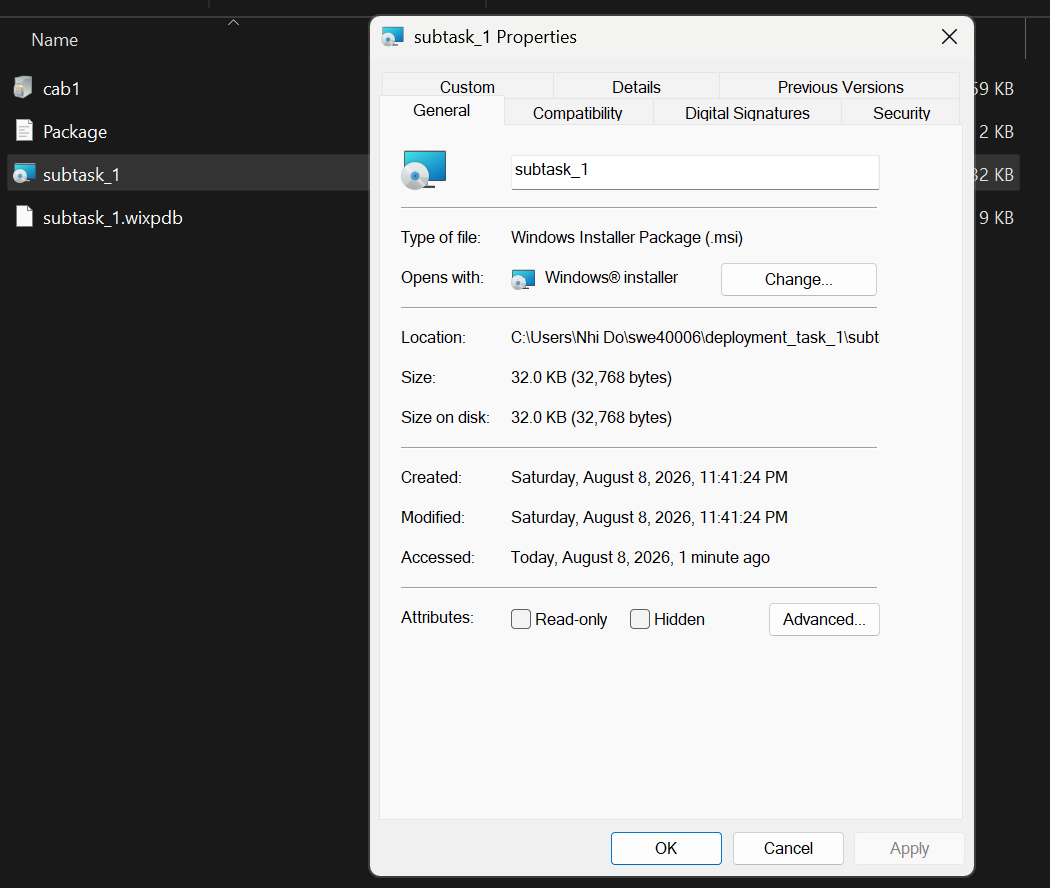
\includegraphics[scale=0.4]{images/1_msi.jpg}
\vspace{-1em}
\caption{The MSI file is created.}
\end{figure}

Running the installer \texttt{subtask\_1.msi} installs the application. The screenshot below shows that the app is successfully installed in the Program Files(x86) folder and runs as expected.

\begin{figure}[H]
\centering
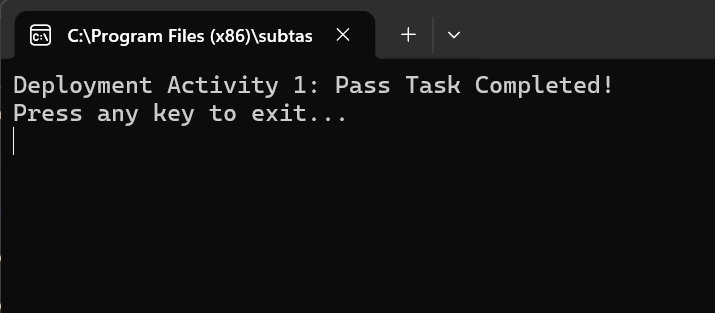
\includegraphics[scale=0.5]{images/1_run_app.jpg}
\vspace{-1em}
\caption{Running the console application after it has been installed.}
\end{figure}

The application Subtask 1 is finally uninstalled.

\begin{figure}[H]
\centering
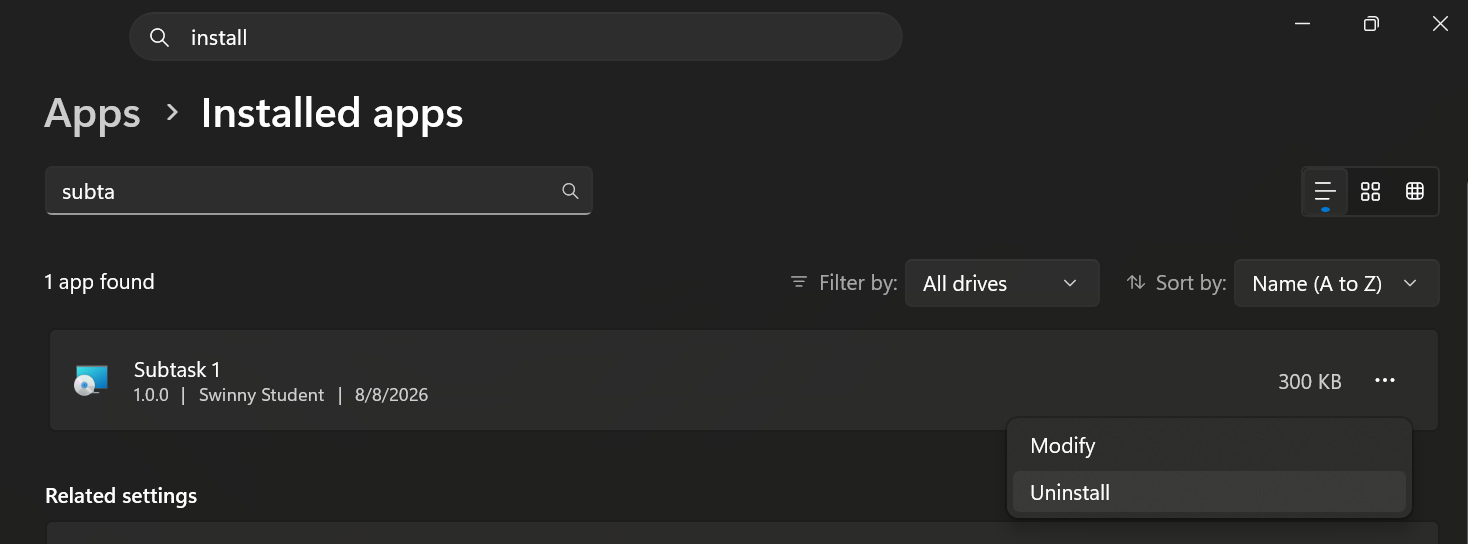
\includegraphics[scale=0.5]{images/1_uninstall_app.jpg}
\vspace{-1em}
\caption{Uninstalling the application.}
\end{figure}

\subsection{Task 1.2}

For task 1.2, I built and packaged a C++ console grading application also using the WiX toolset.

First, I created the program and built it in Release mode. The resulting executable code is created in the \texttt{x64} directory.

\begin{figure}[H]
\centering
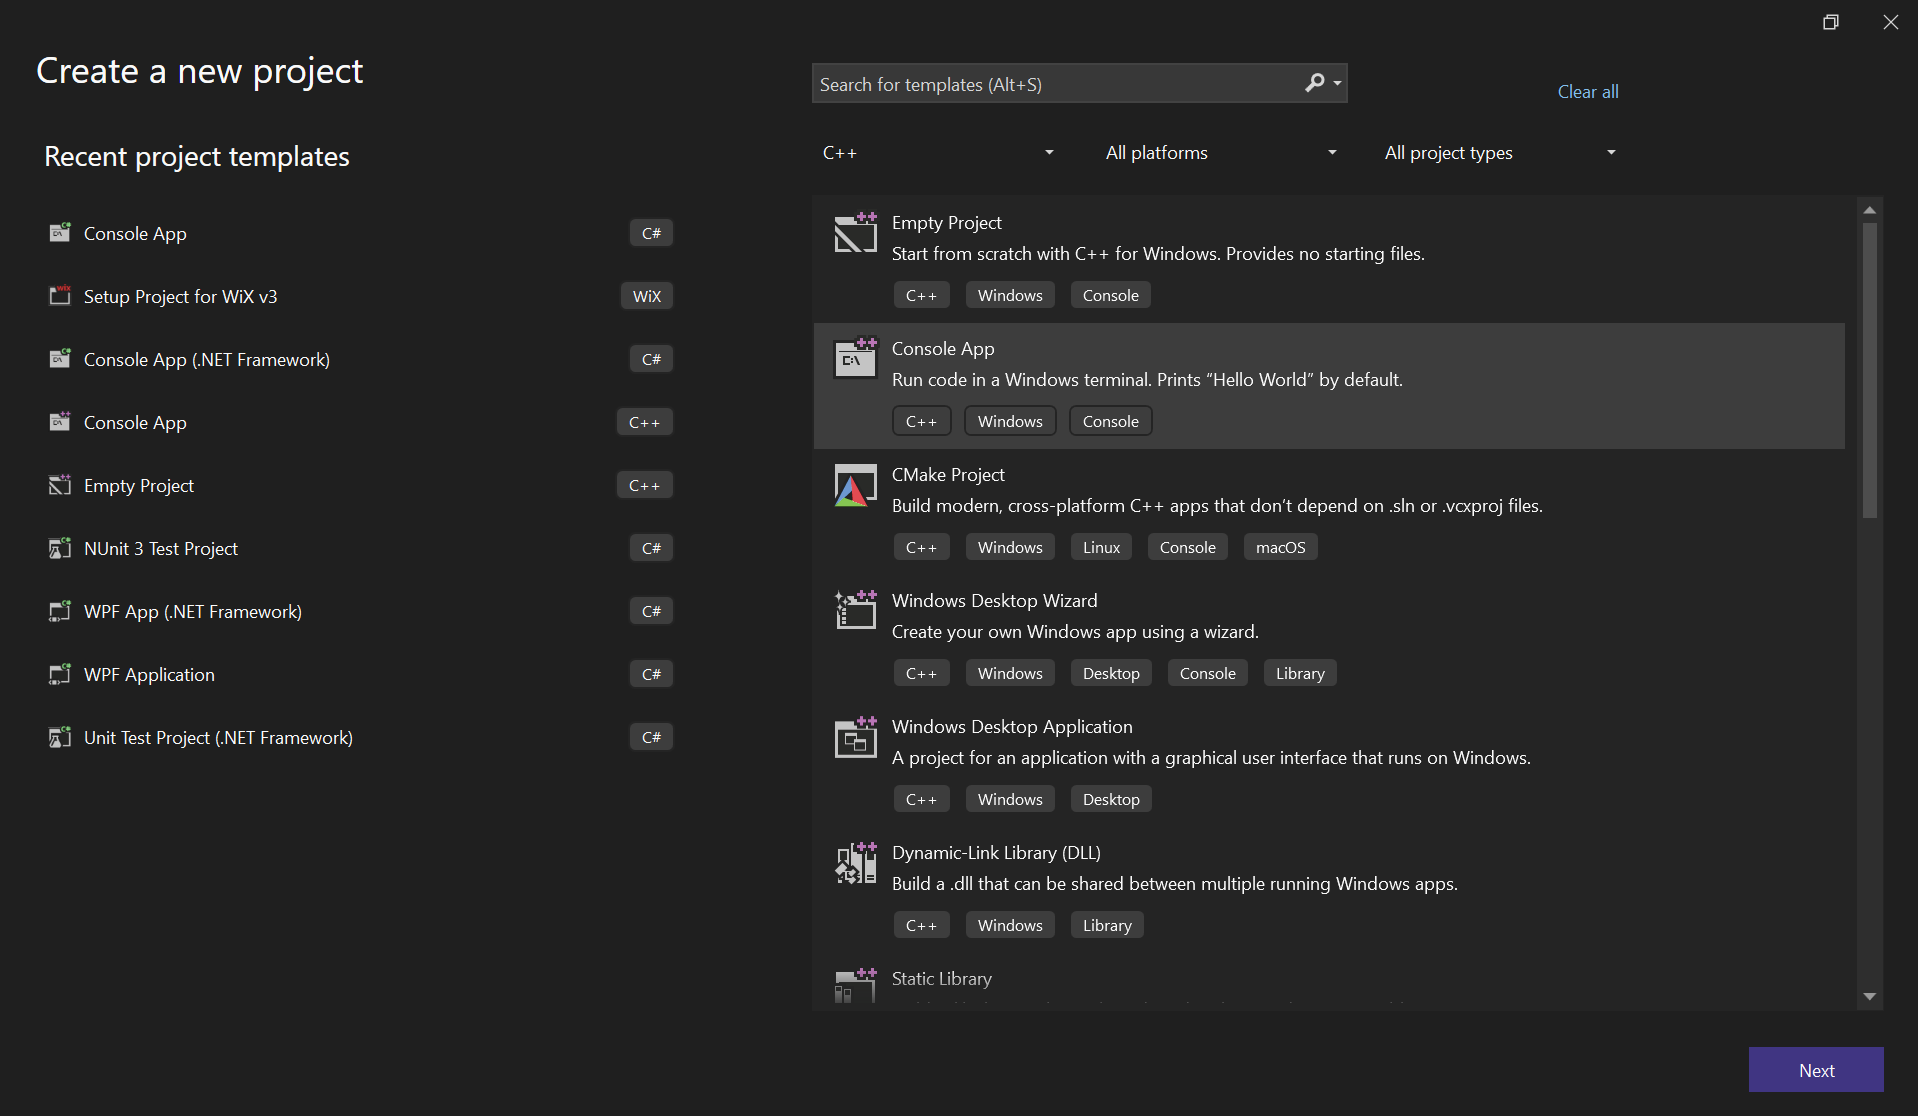
\includegraphics[scale=0.4]{images/2_create_project.jpg}
\vspace{-1em}
\caption{Creating a new C++ console application.}
\end{figure}

\begin{figure}[H]
\centering
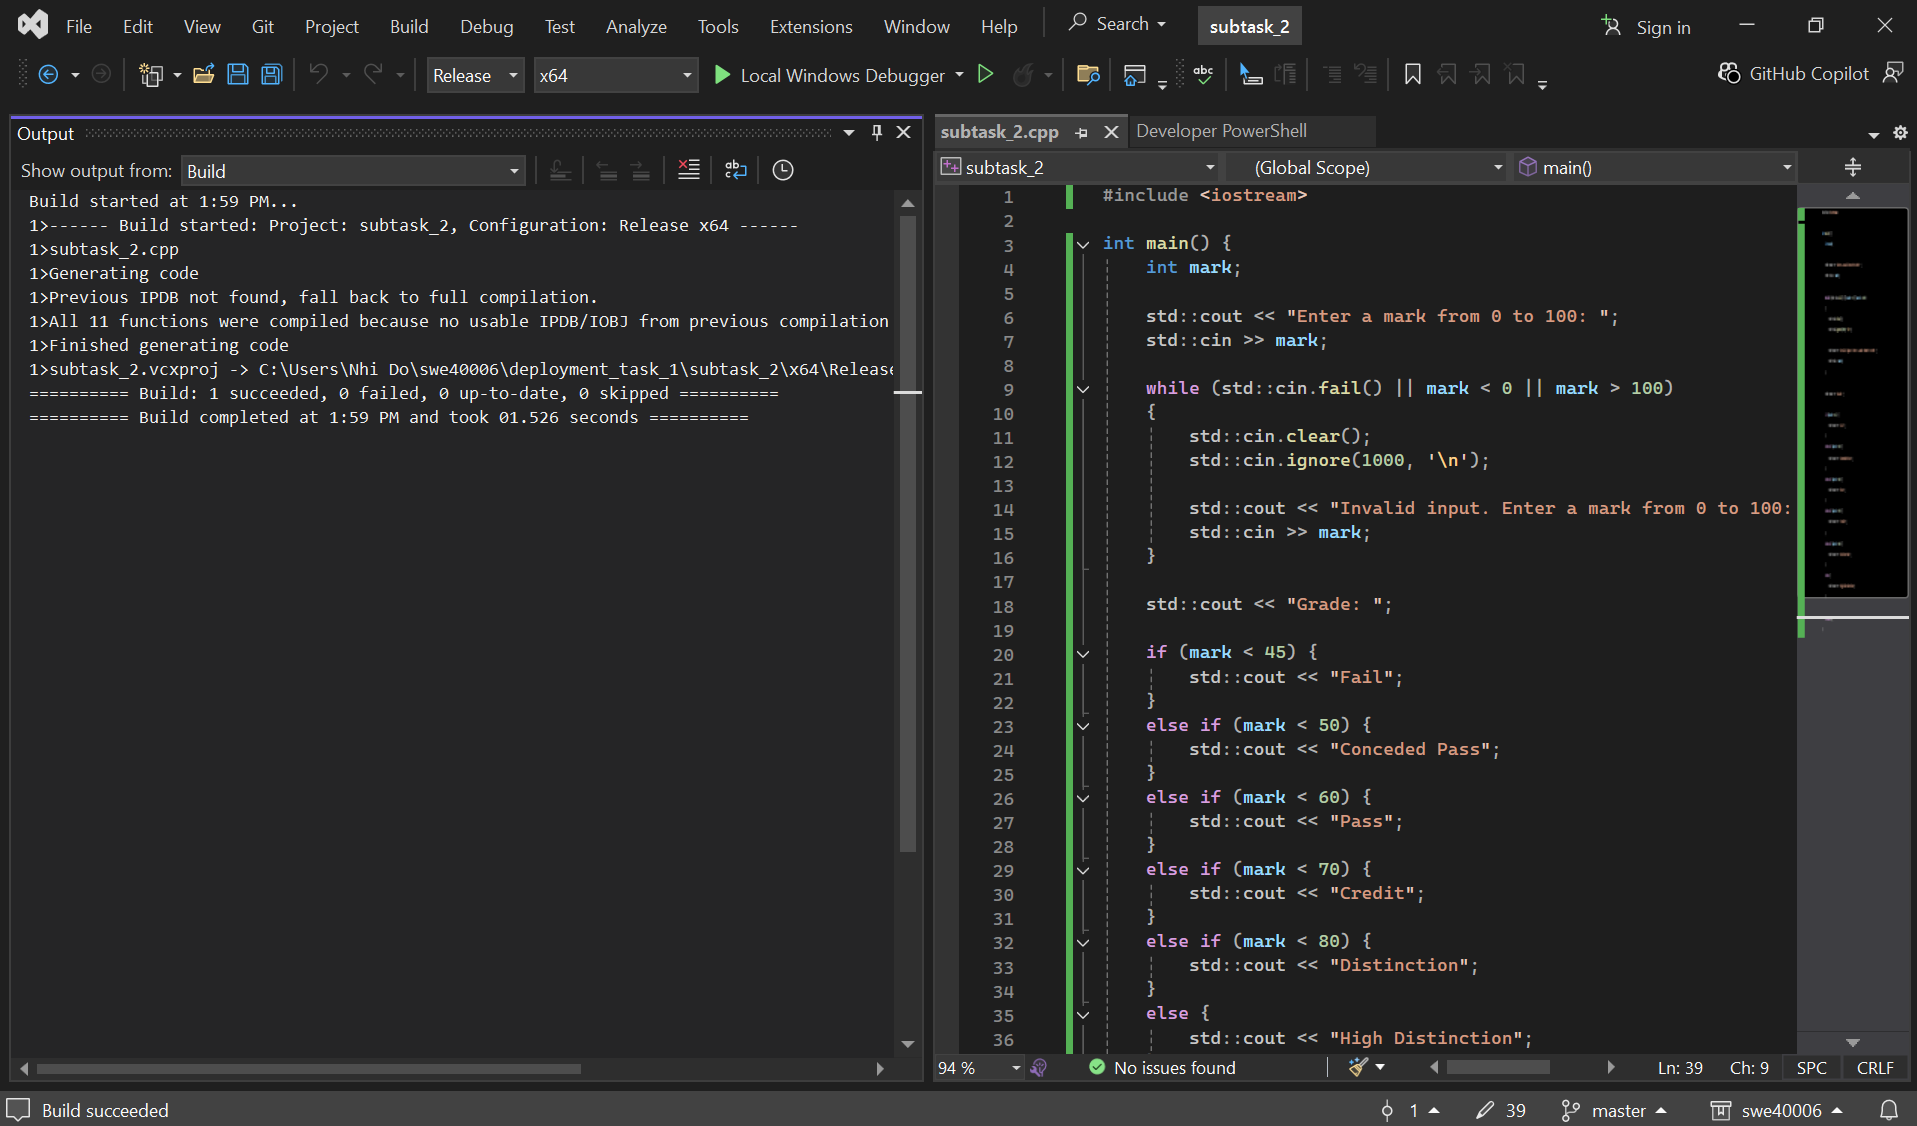
\includegraphics[scale=0.4]{images/2_build_project.jpg}
\vspace{-1em}
\caption{Building the project in Release mode.}
\end{figure}

\begin{figure}[H]
\centering
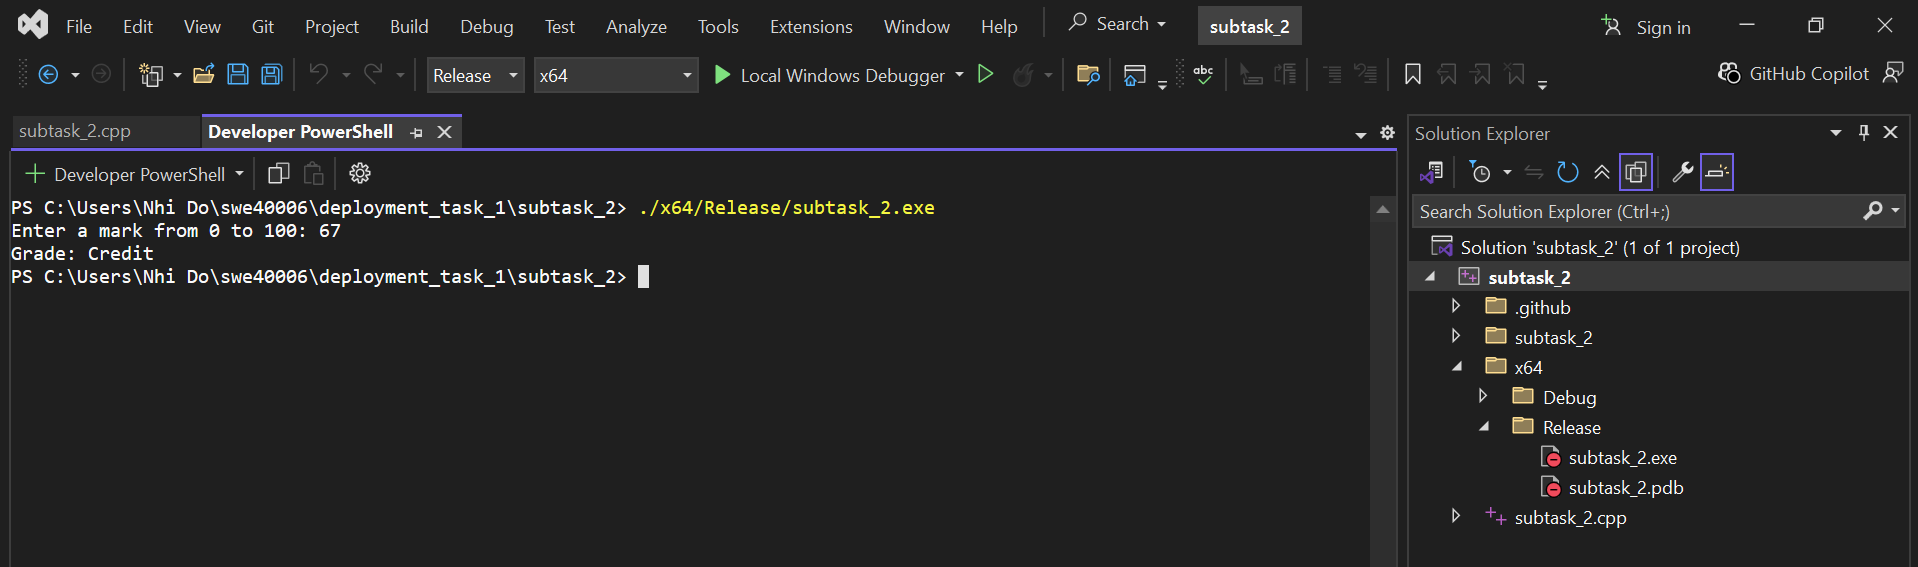
\includegraphics[scale=0.4]{images/2_run_project.jpg}
\vspace{-1em}
\caption{Verifying that the executable exists and runs correctly. The executable is created in the \texttt{x64/Release} directory as seen in the Solution Explorer.}
\end{figure}

Similarly, a WiX installer application is created, and a \texttt{.wxs} file is written to configure the installer.

\begin{figure}[H]
\centering
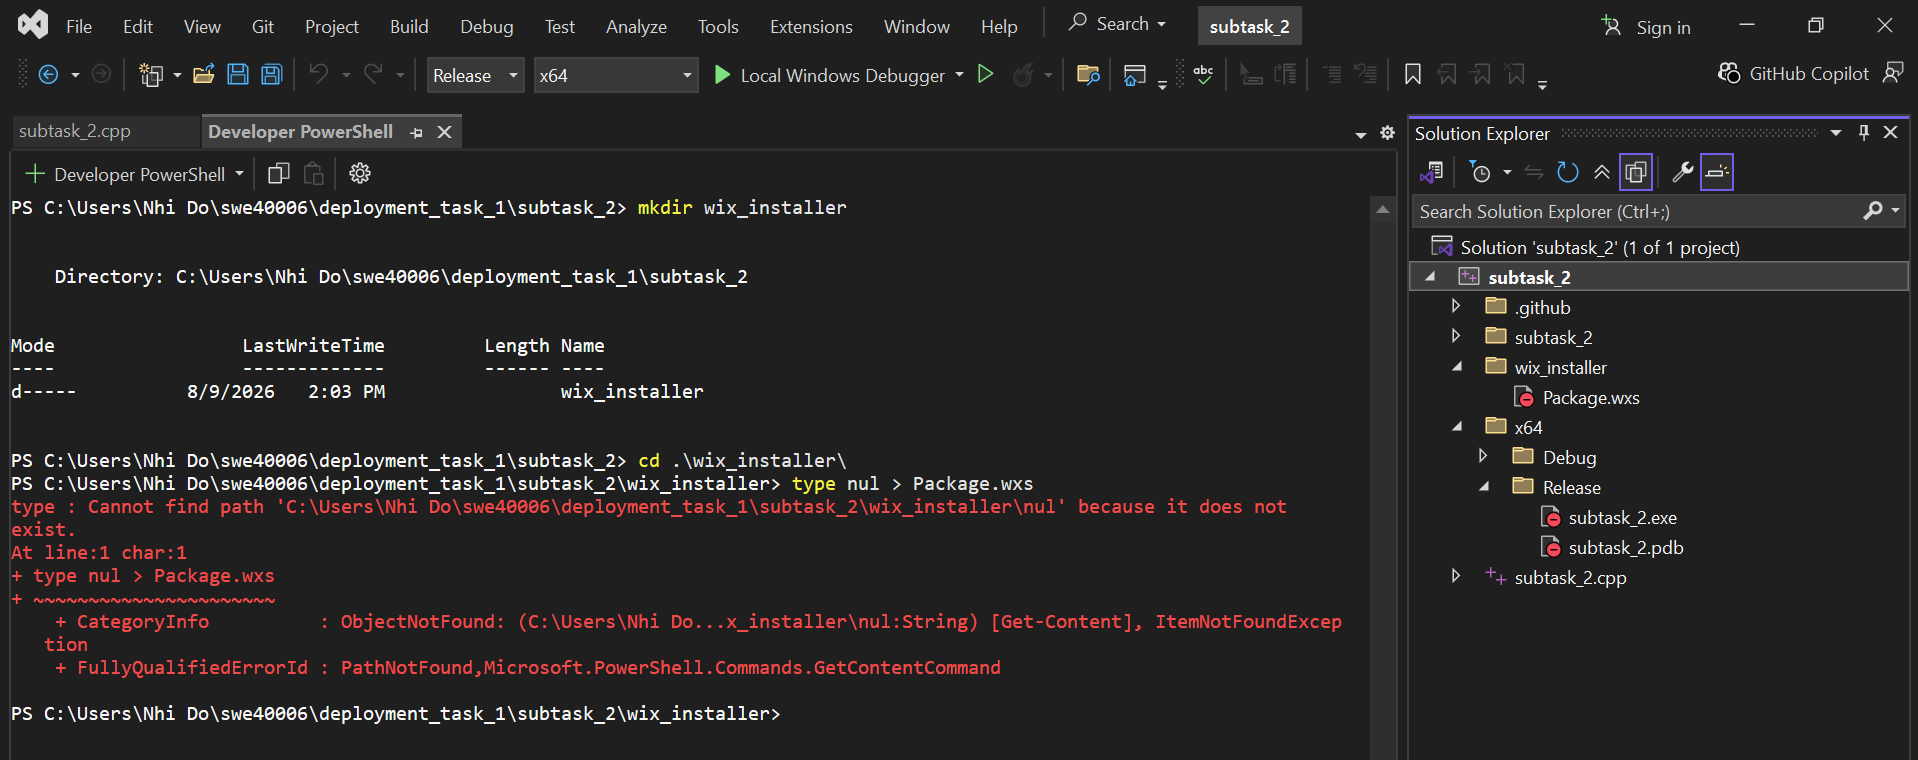
\includegraphics[scale=0.4]{images/2_create_wix.jpg}
\vspace{-1em}
\caption{Creating the WiX installer project and source file.}
\end{figure}

\begin{figure}[H]
\centering
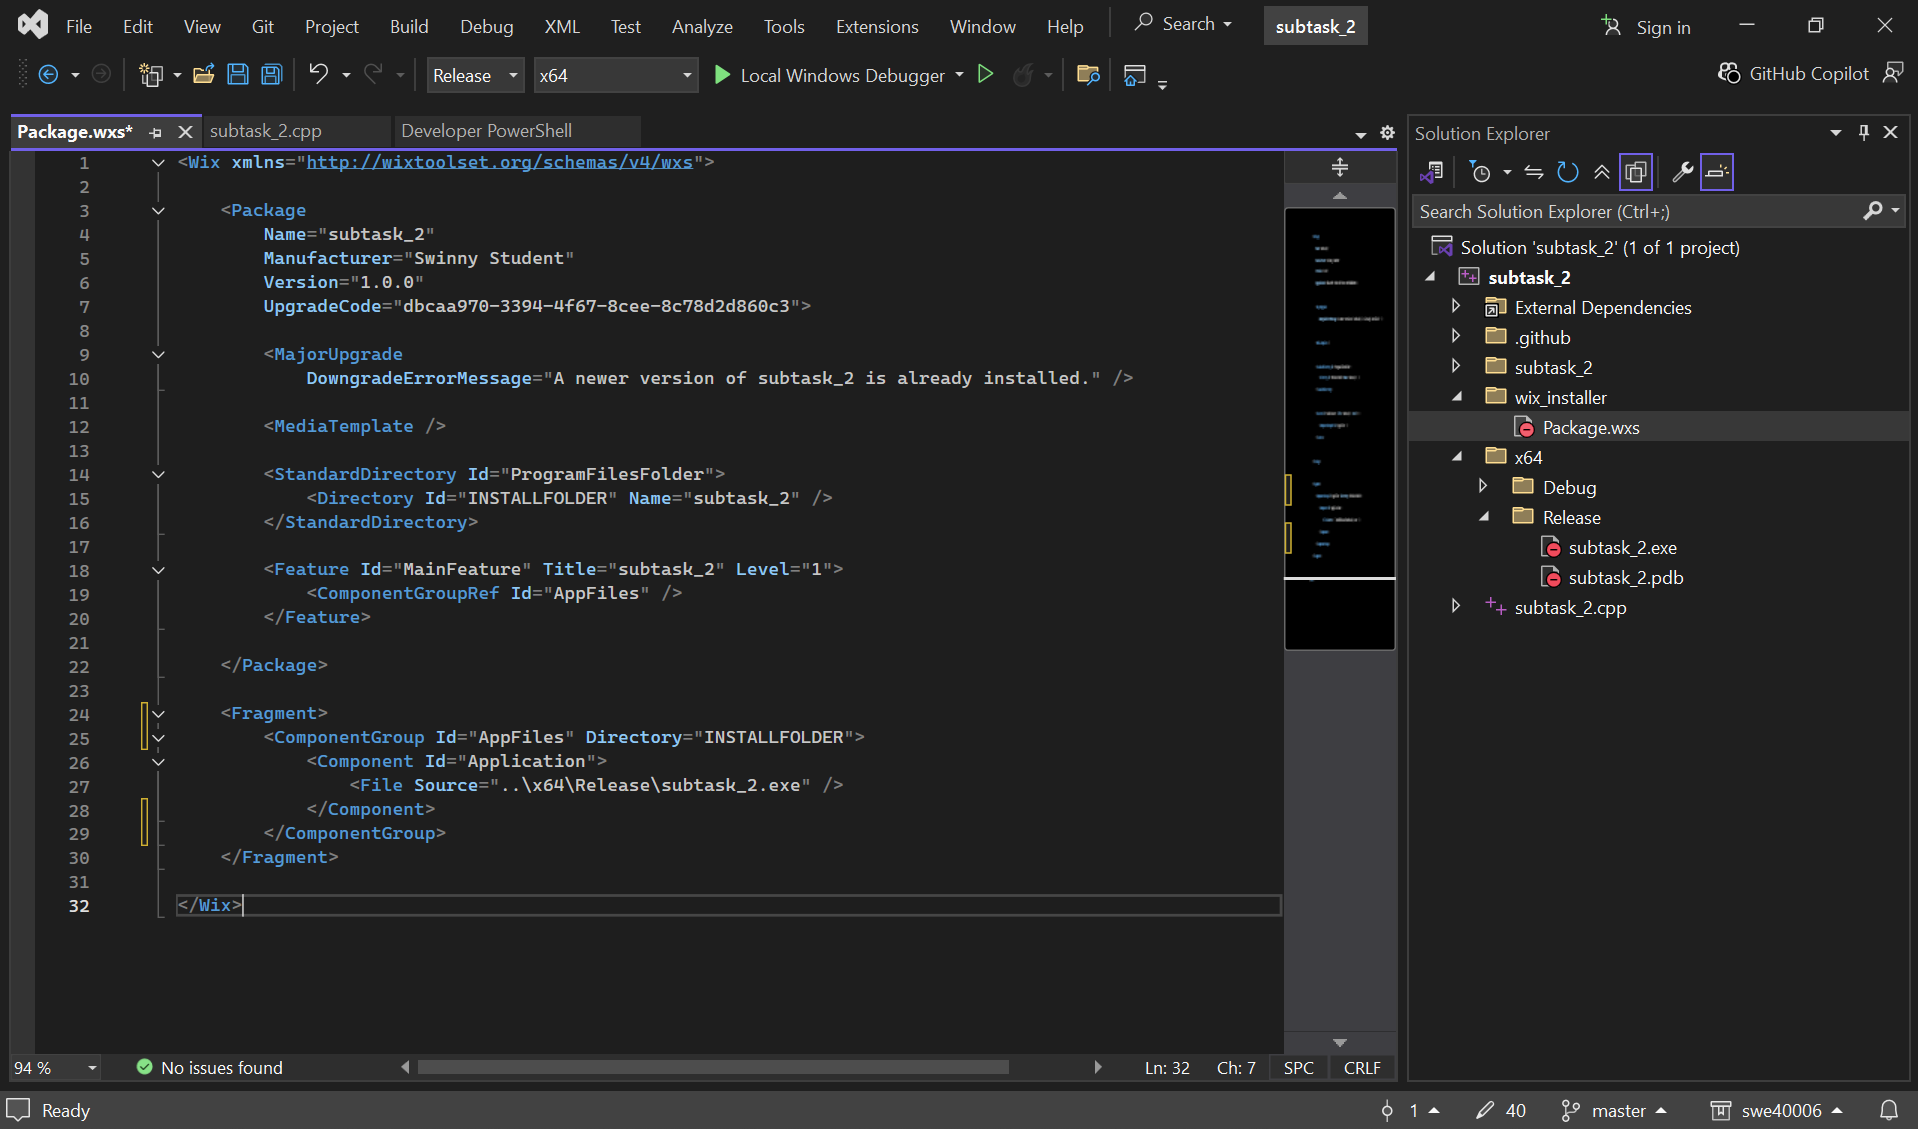
\includegraphics[scale=0.4]{images/2_create_wxs.jpg}
\vspace{-1em}
\caption{Writing the \texttt{.wxs} file.}
\end{figure}

\begin{figure}[H]
\centering
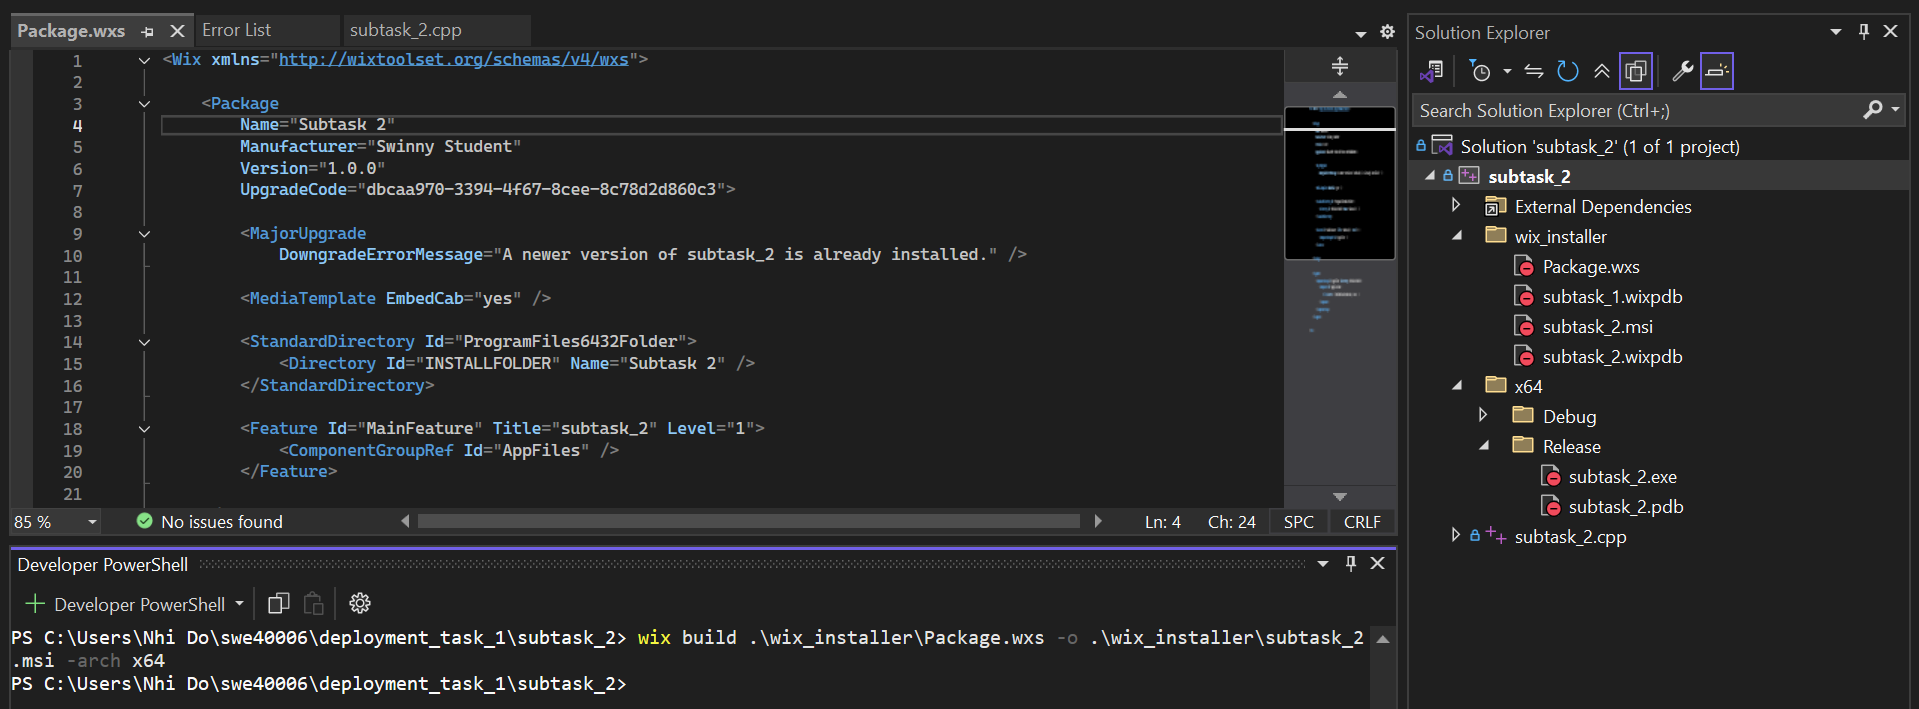
\includegraphics[scale=0.4]{images/2_build_msi.jpg}
\vspace{-1em}
\caption{Building the MSI package.}
\end{figure}

Running the MSI package installs the app in the Program Files(x86) folder. The application runs as intended.

\begin{figure}[H]
\centering
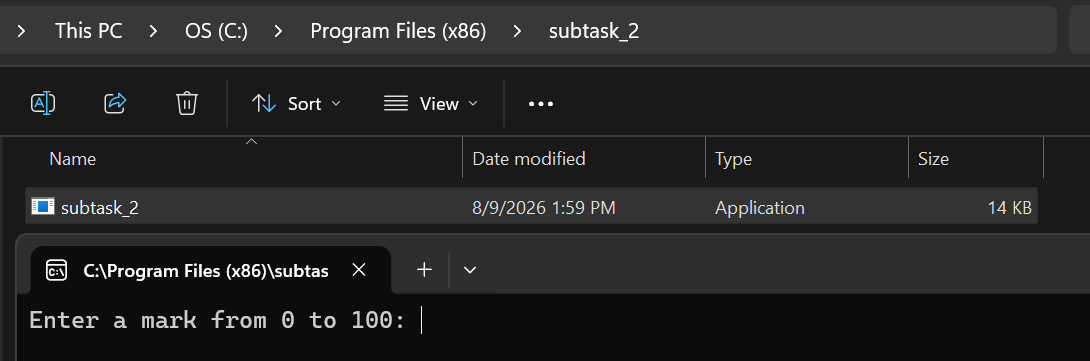
\includegraphics[scale=0.4]{images/2_run_app.jpg}
\vspace{-1em}
\caption{The application is installed in the Program Files (x86) folder. Double-clicking the app executes the program.}
\end{figure}

\begin{figure}[H]
\centering
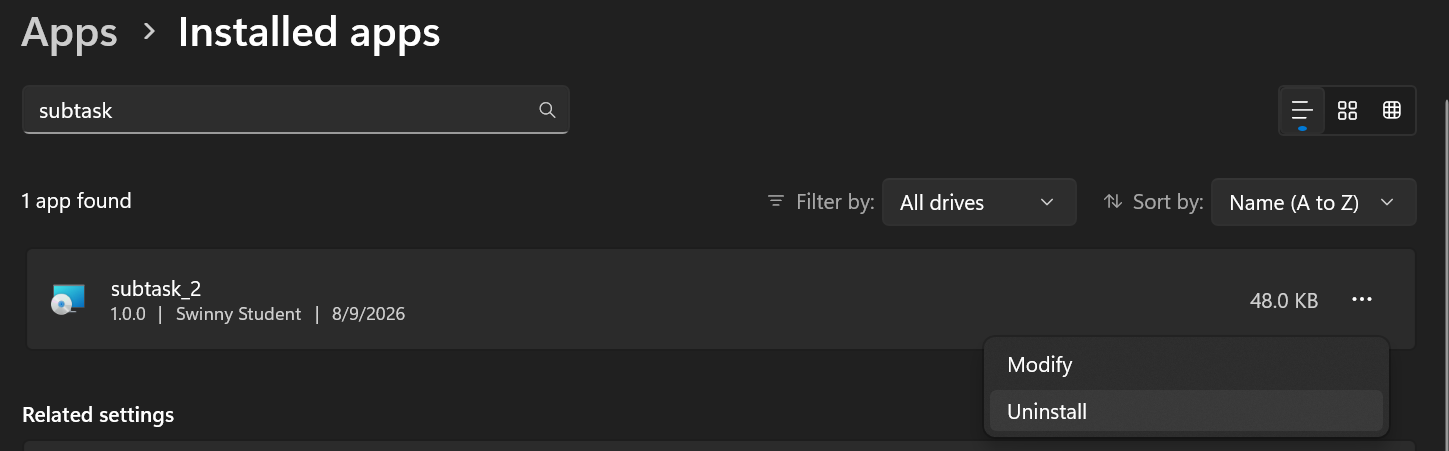
\includegraphics[scale=0.4]{images/2_uninstall_app.jpg}
\vspace{-1em}
\caption{Uninstalling the application.}
\end{figure}

\subsection{Task 1.3}
The application created for subtask 1.3 is a simple WinForms application, making the use of the packages \texttt{Newtonsoft.Json} and \texttt{Serilog} to demonstrate the packaging of multiple external DLLs.

First, I created the WinForms application using the template provided in Visual Studio.

\begin{figure}[H]
\centering
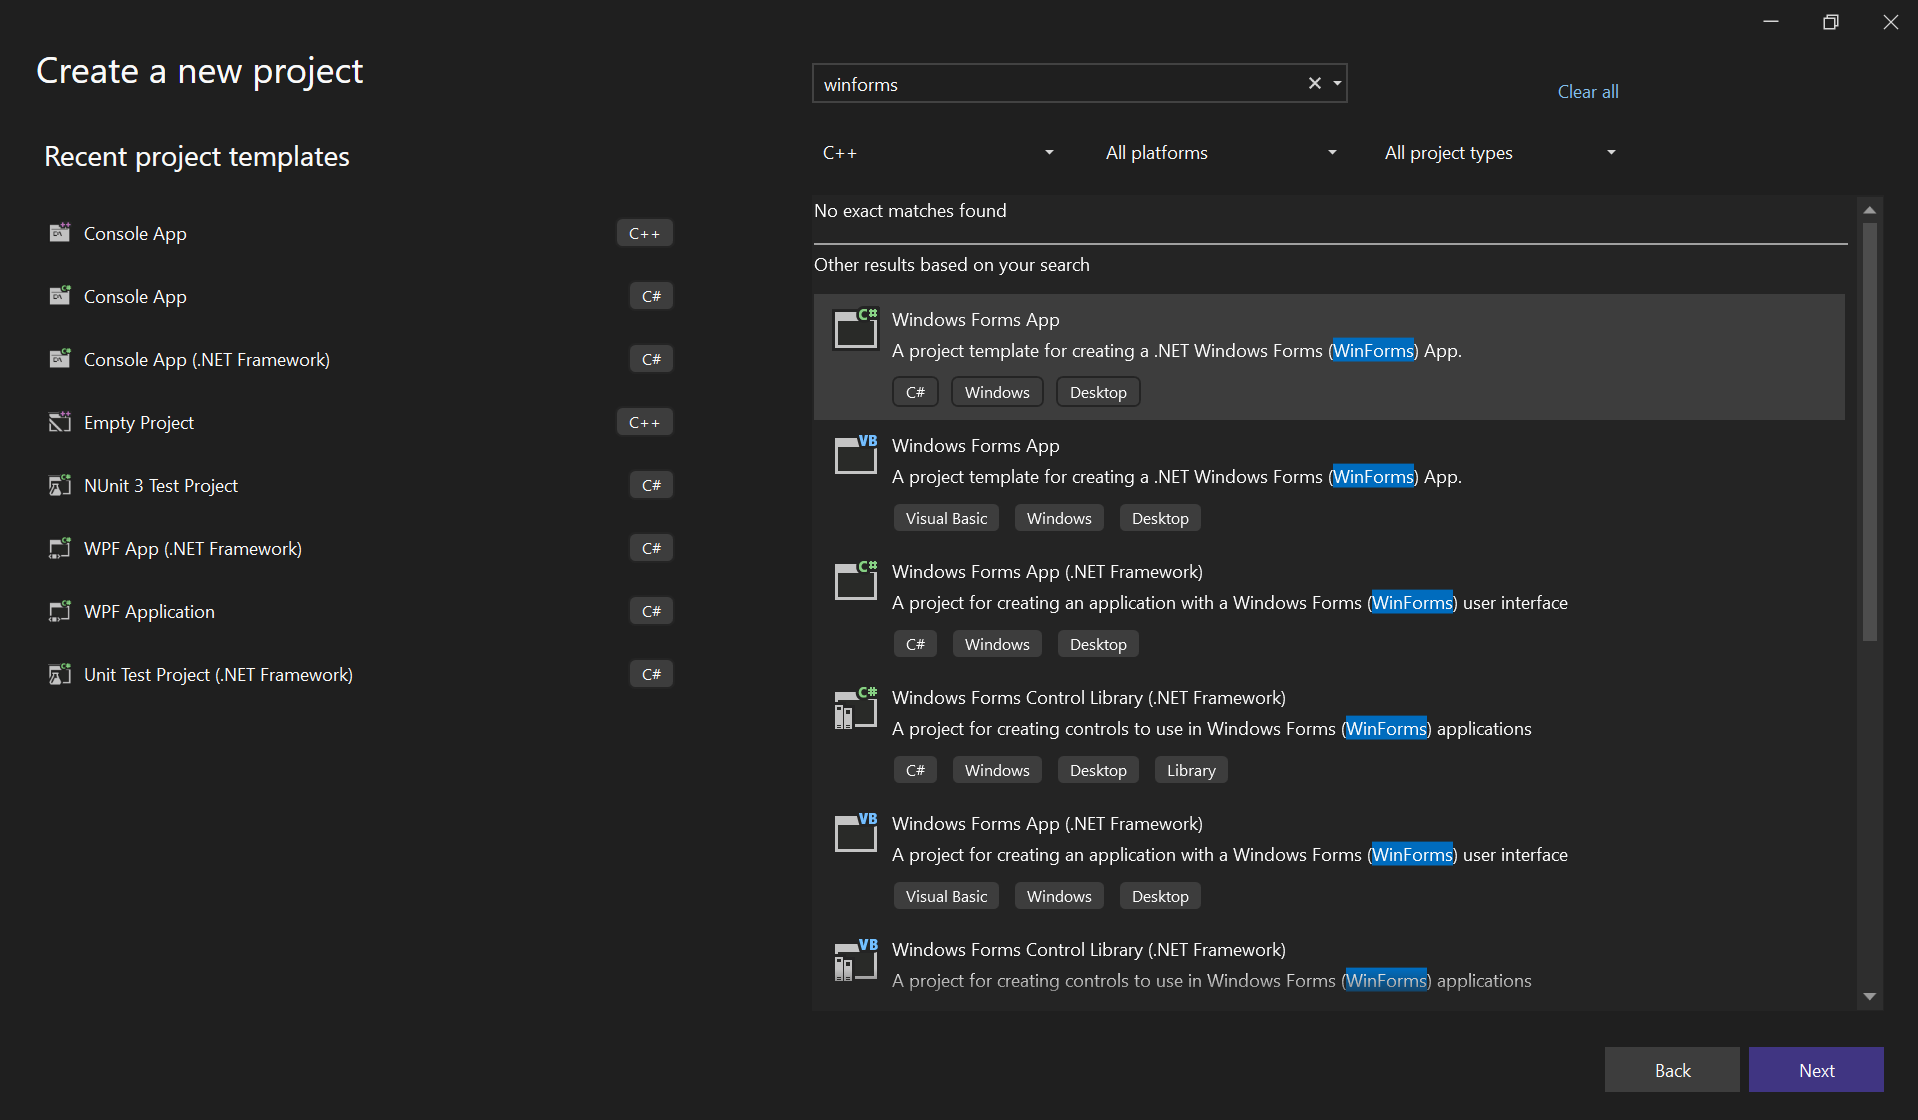
\includegraphics[scale=0.4]{images/3_create_project.jpg}
\vspace{-1em}
\caption{Creating a new WinForms project.}
\end{figure}

The application simply displays a window with a button which shows a messages and logs some information when it is clicked. The screenshot below shows that it compiles and runs successfully.

\begin{figure}[H]
\centering
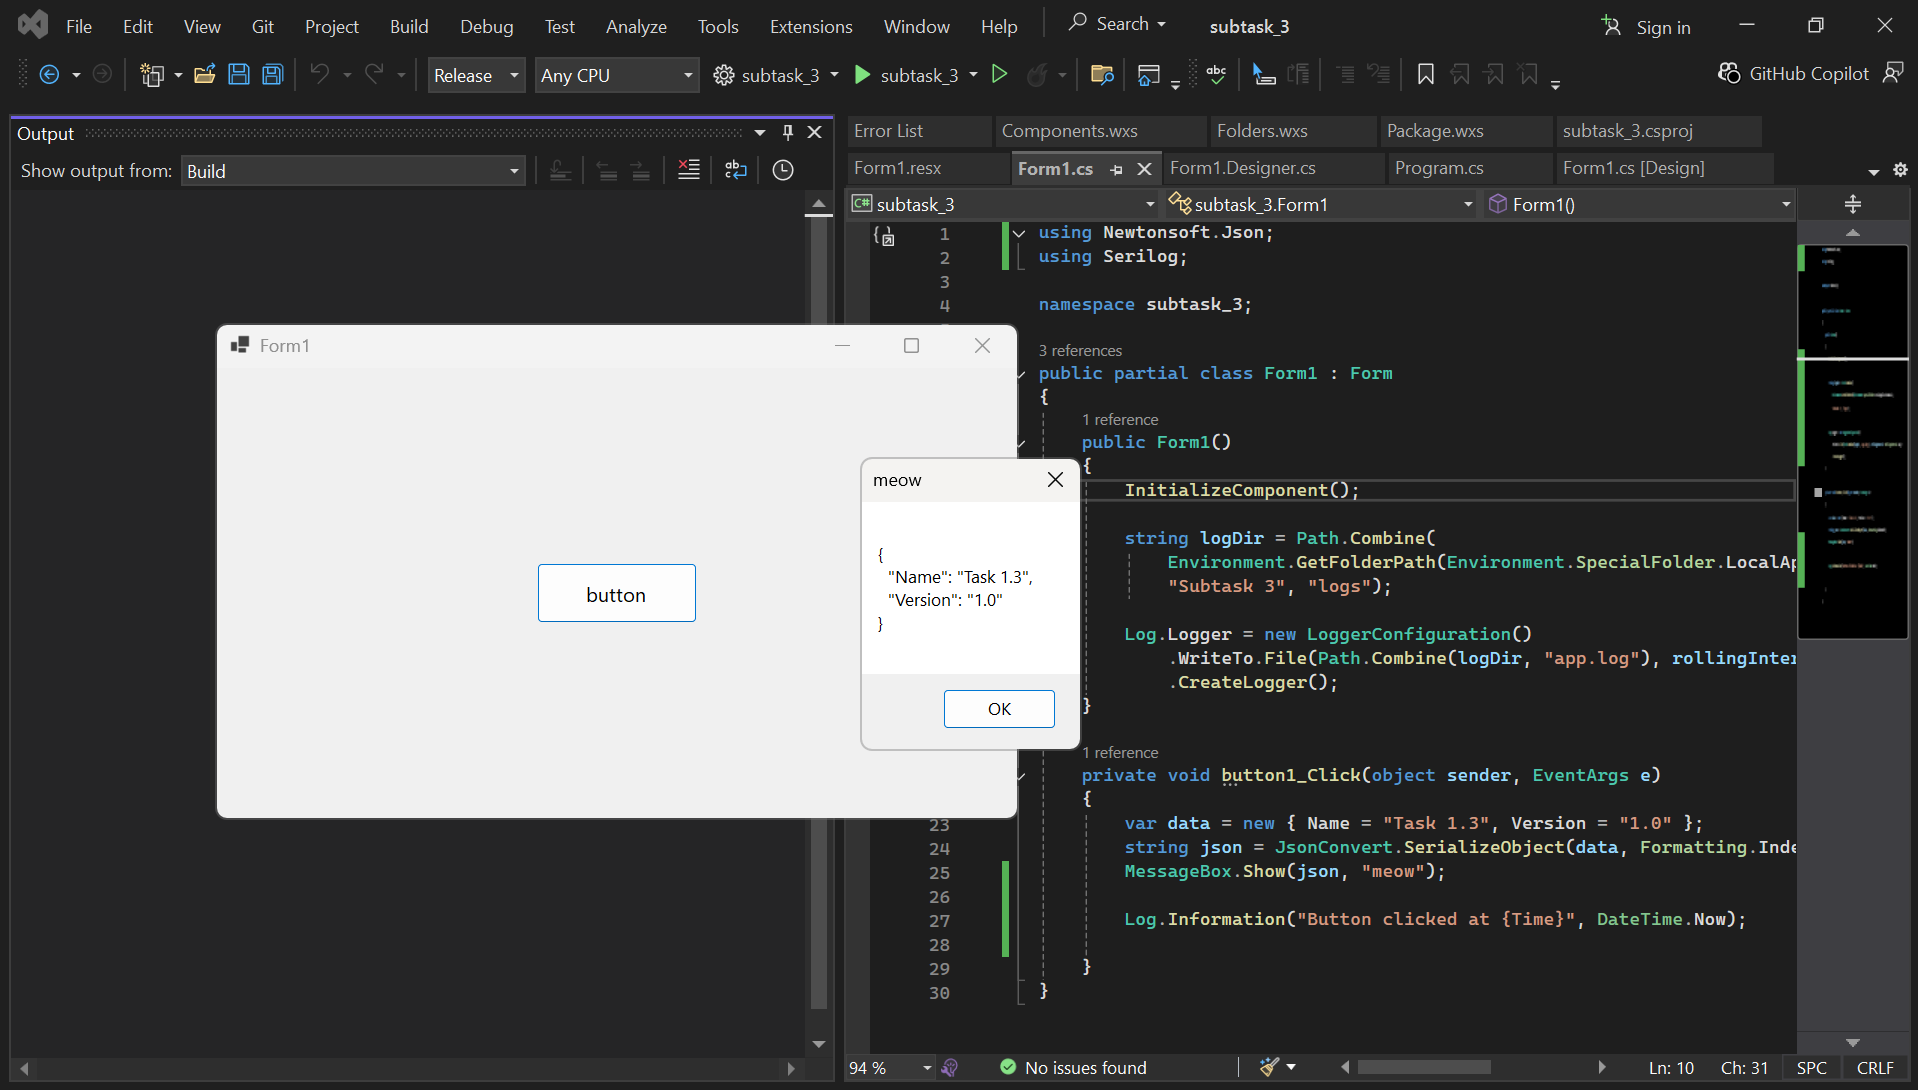
\includegraphics[scale=0.4]{images/3_build_project.jpg}
\vspace{-1em}
\caption{The app successfully runs.}
\end{figure}

\begin{figure}[H]
\centering
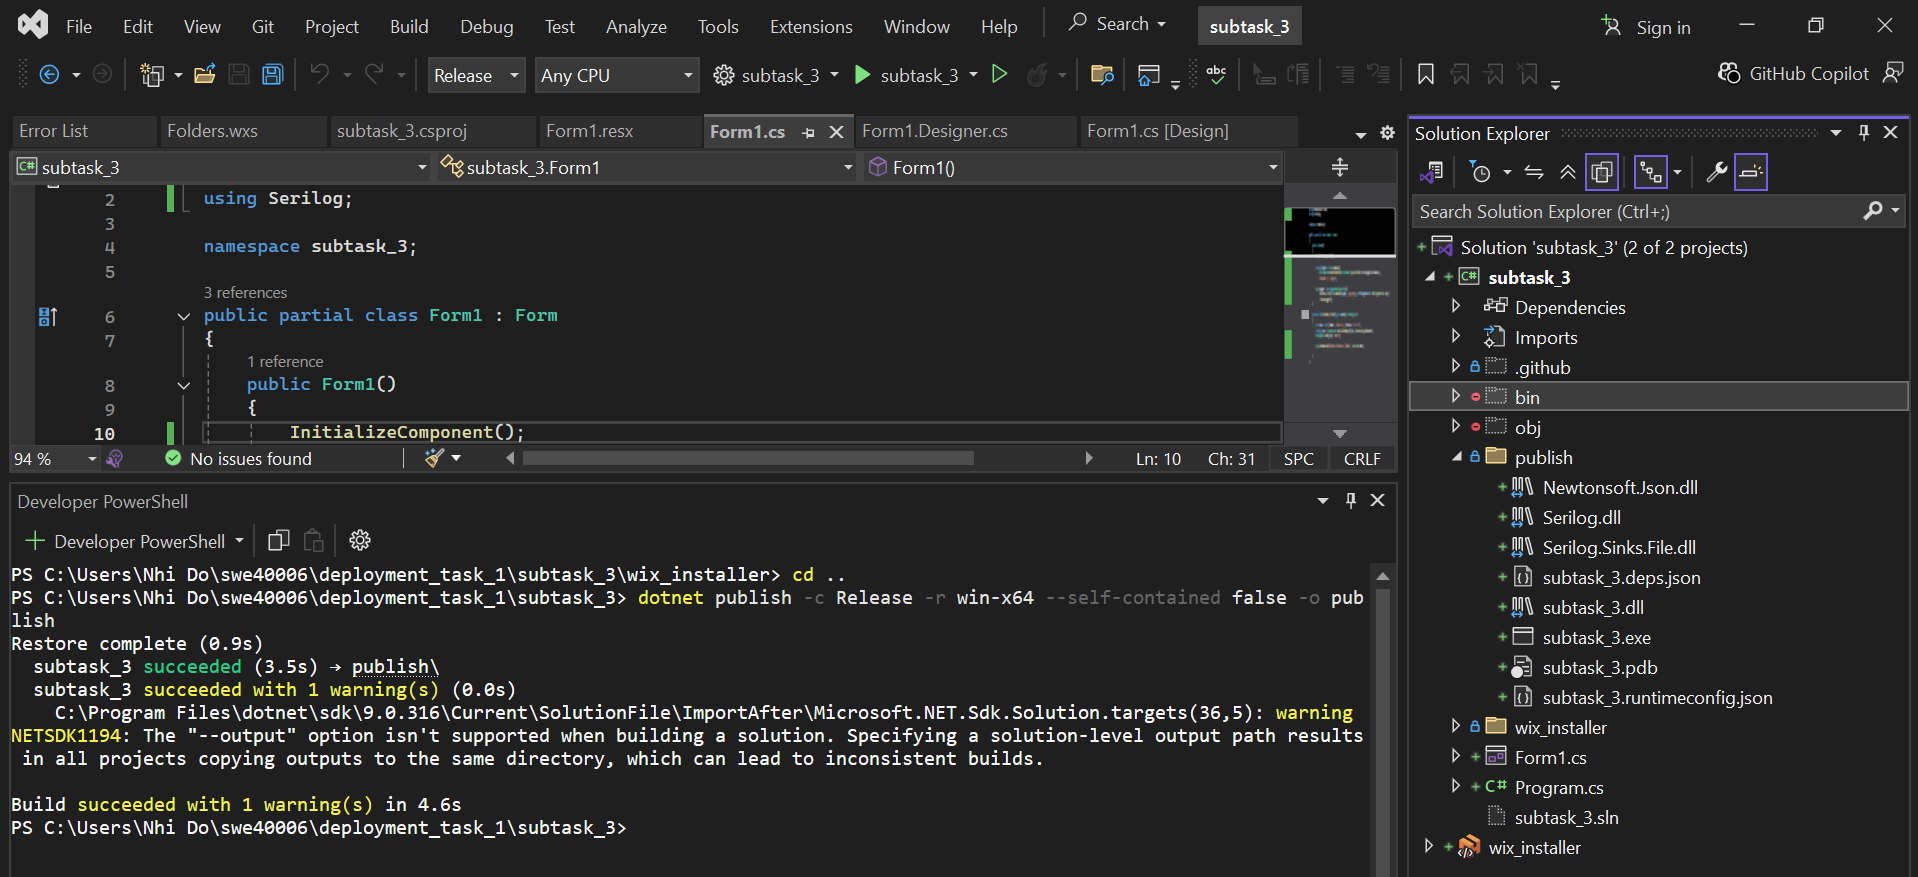
\includegraphics[scale=0.4]{images/3_publish_project.jpg}
\vspace{-1em}
\caption{The project is published into a \texttt{publish} directory The Solution Explorer on the right shows that the executable, runtime dependencies, and DLLs were created.}
\end{figure}

Next, I created a new WiX project, this time using the template provided by the HeatWave extension.

\begin{figure}[H]
\centering
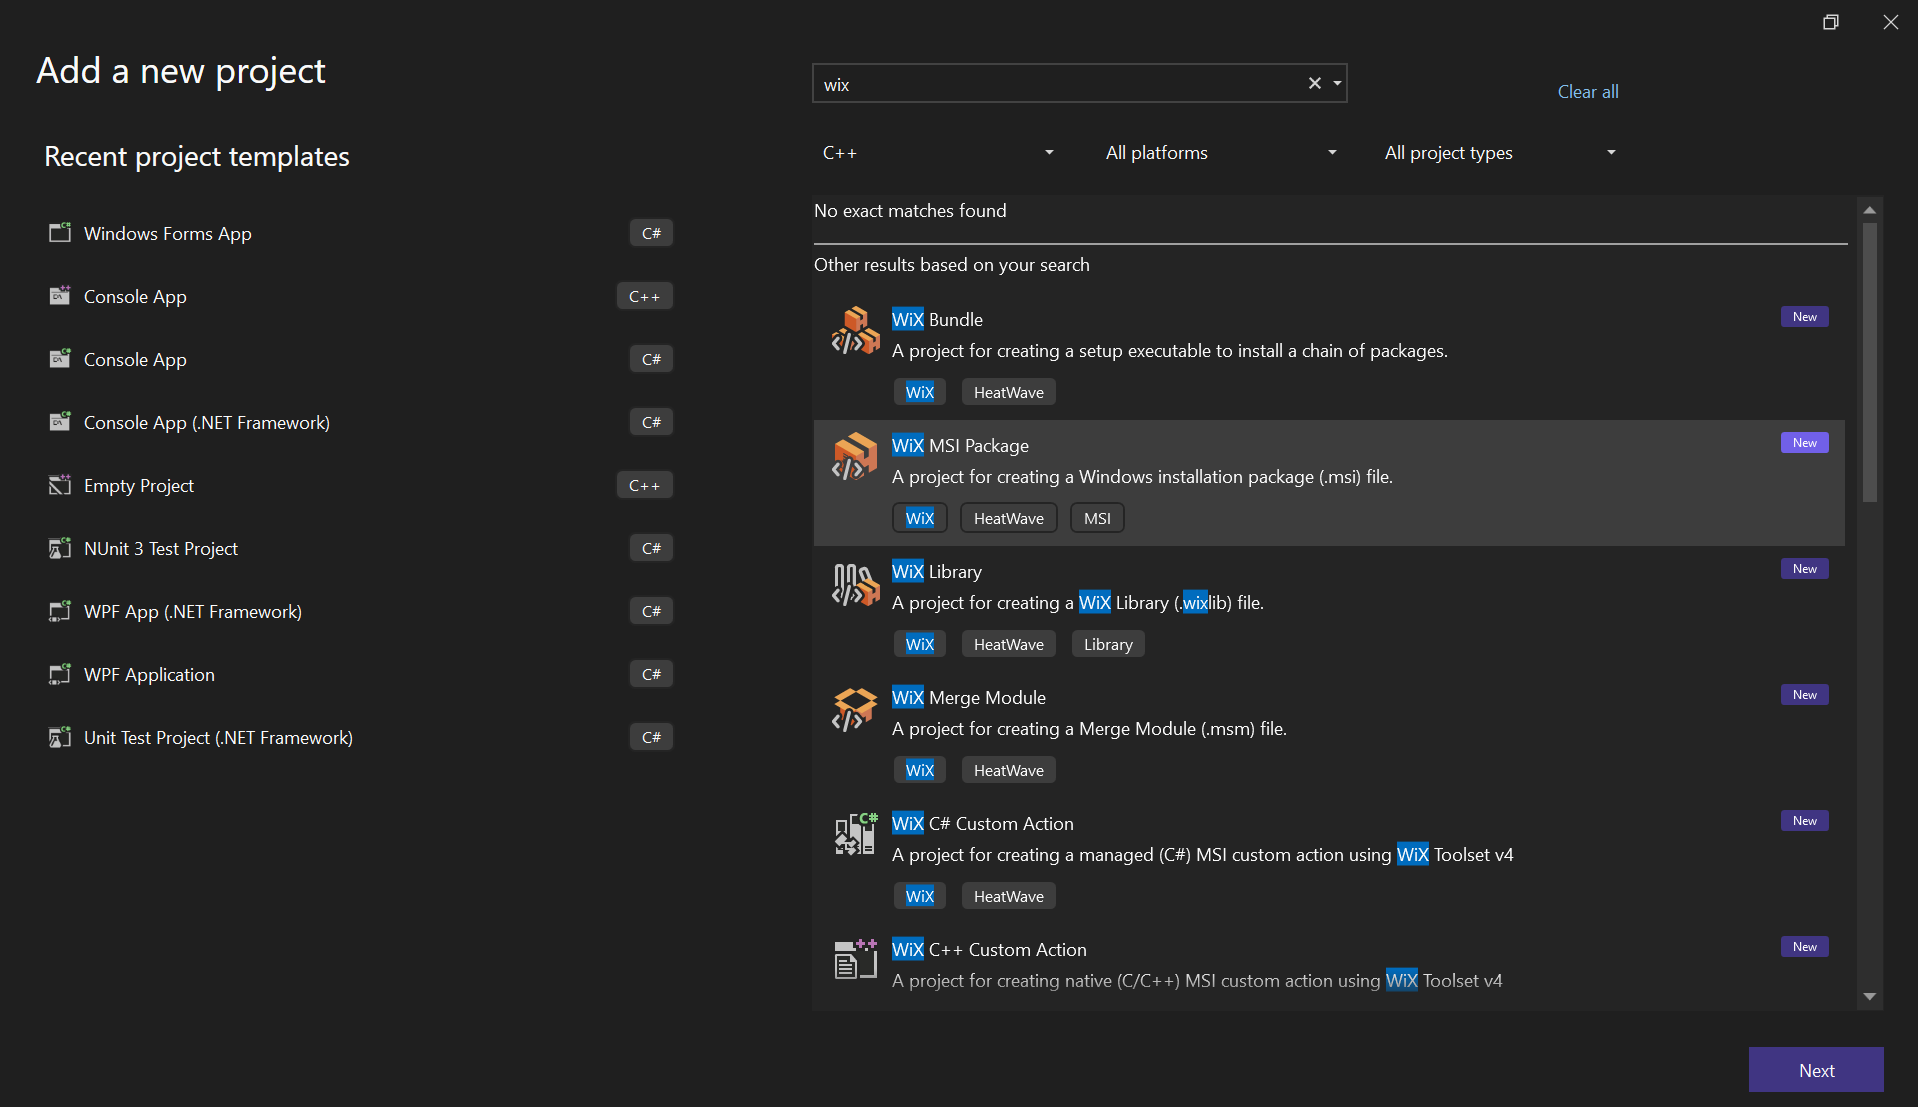
\includegraphics[scale=0.4]{images/3_create_wix.jpg}
\vspace{-1em}
\caption{Creating a new WiX MSI Package project.}
\end{figure}

The \texttt{Components.wxs} file was configured to include the build outputs. This was done by authoring \texttt{<Component>} tags for each file, including the main executable, the DLL files, and others. Other build configurations were written in \texttt{Package.wxs} and \texttt{Folders.wxs}.

\begin{figure}[H]
\centering
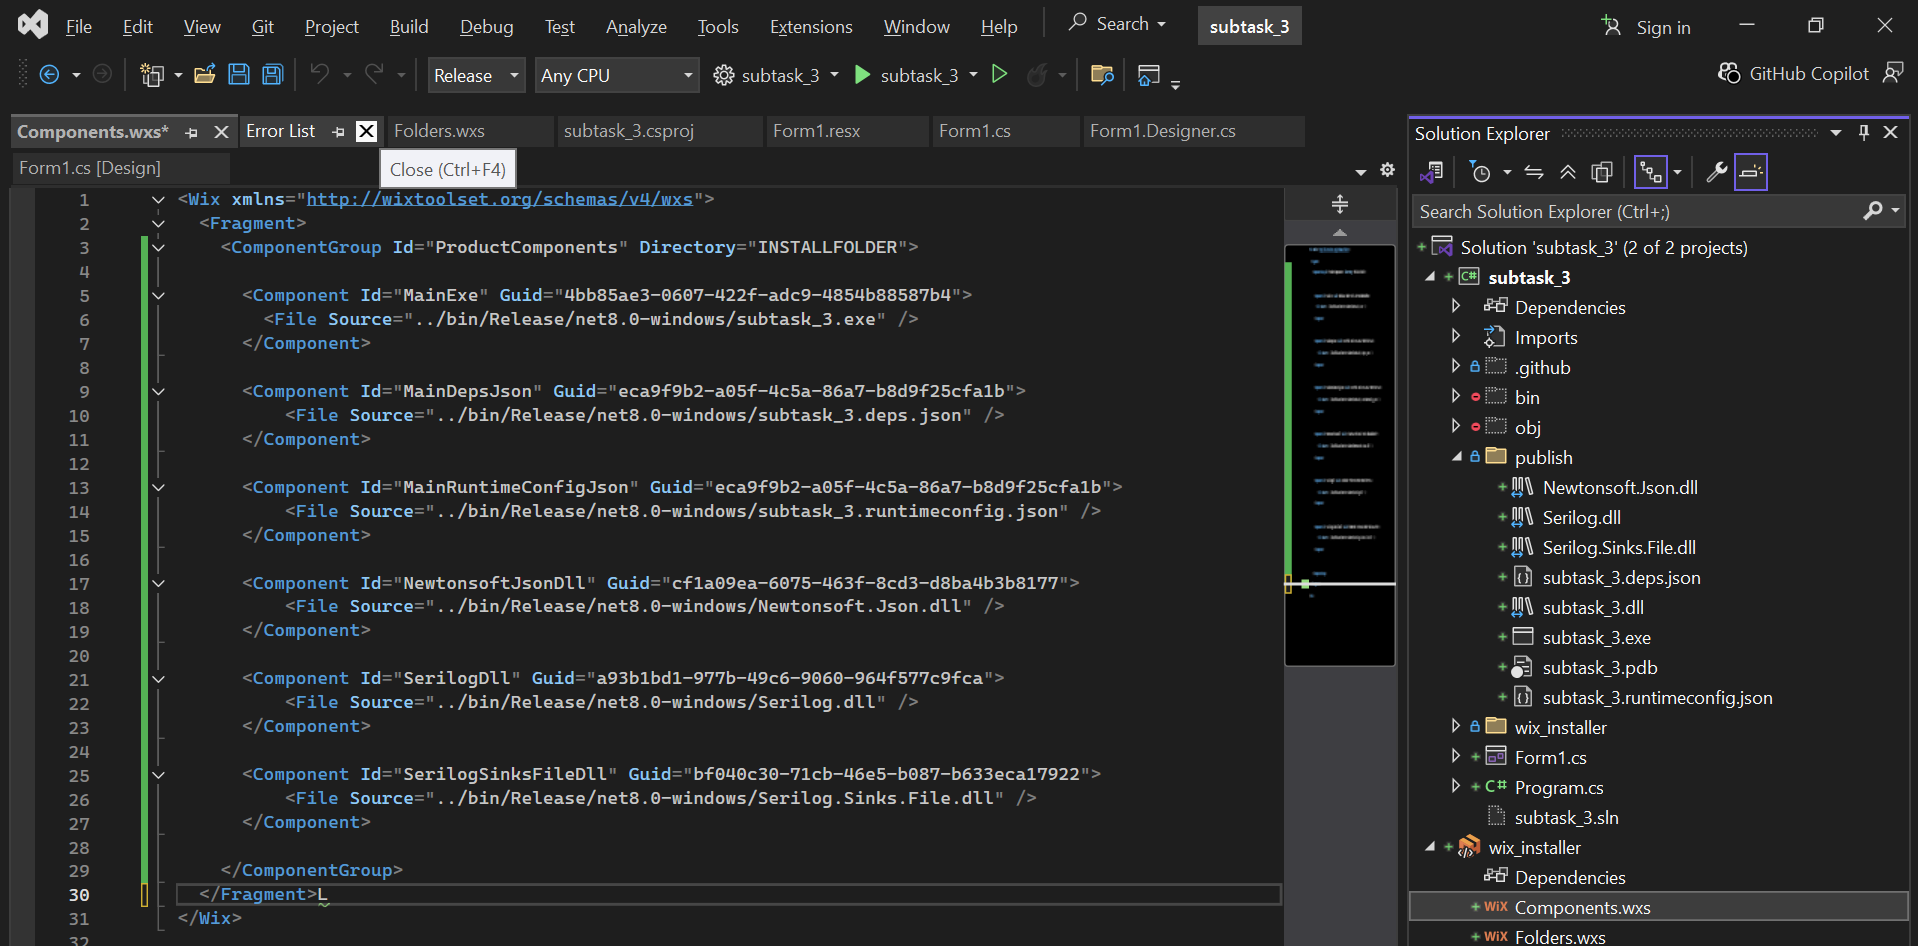
\includegraphics[scale=0.4]{images/3_create_wxs.jpg}
\vspace{-1em}
\caption{Writing the executable, DLLs, and dependencies into the script. These files would be included in the final MSI package.}
\end{figure}

\begin{figure}[H]
\centering
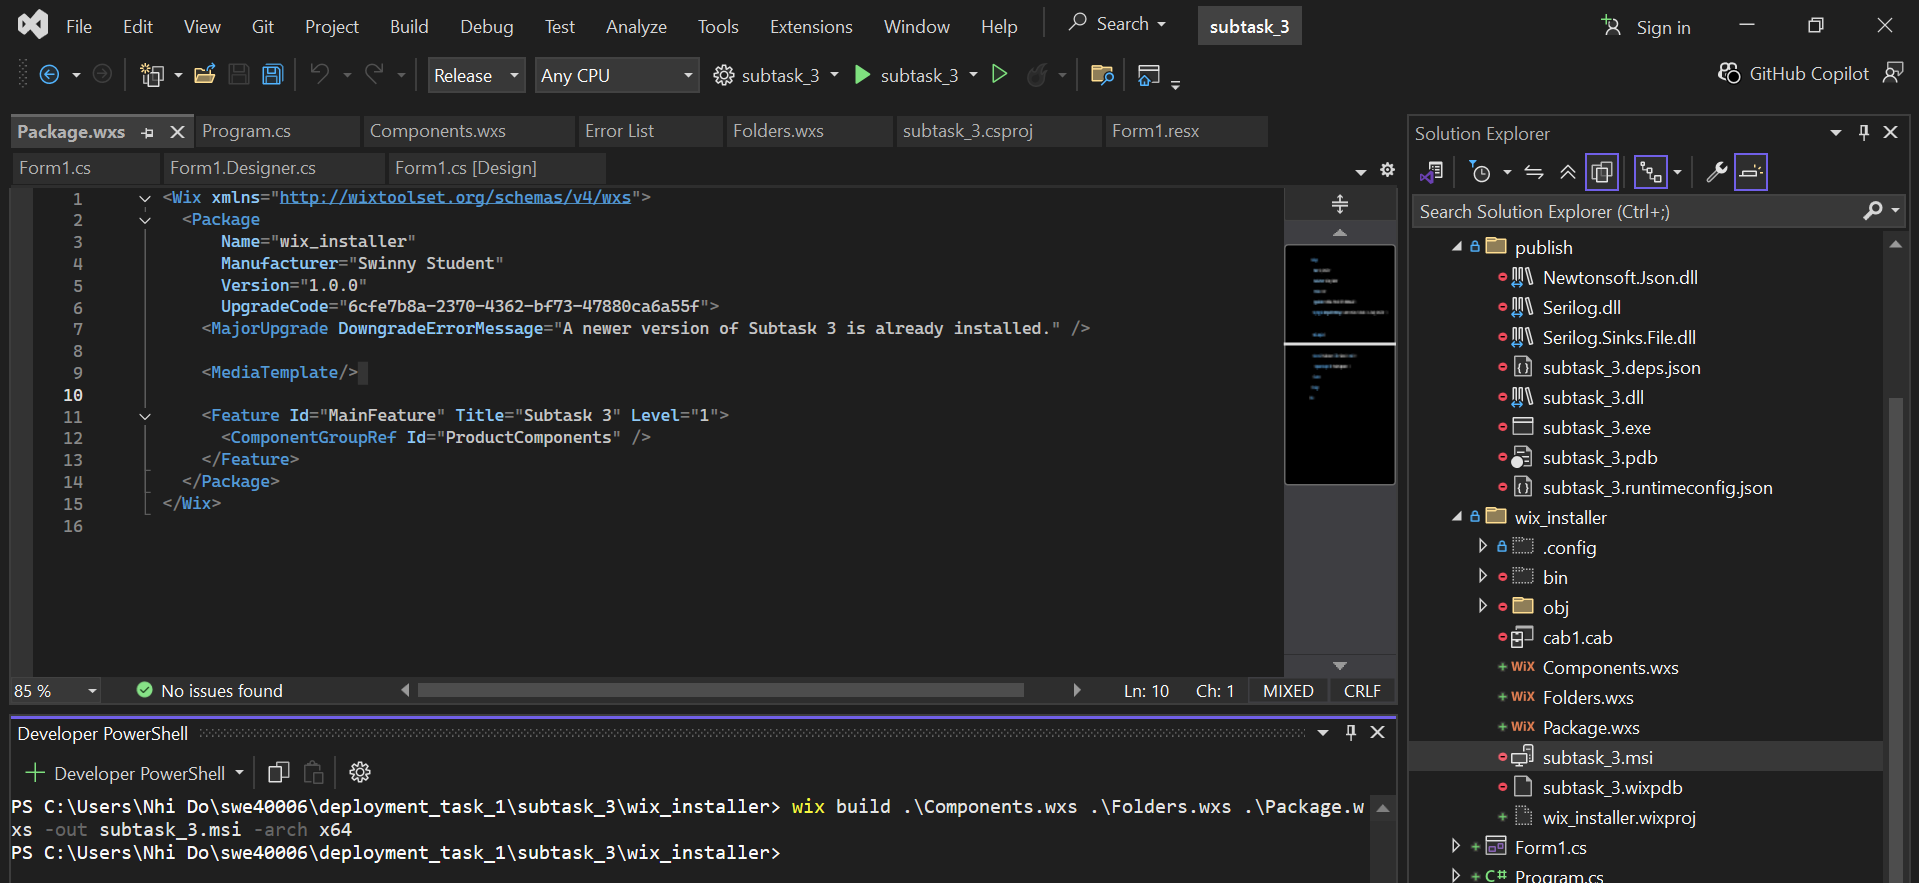
\includegraphics[scale=0.3]{images/3_build_msi.jpg}
\vspace{-1em}
\caption{The WiX project is built to create an MSI package.}
\end{figure}

The application is installed in the Program Files folder, since the platform architecture is specified as 64-bit in the build command this time. The screenshot below proves that the app was installed and executed without any errors.

\begin{figure}[H]
\centering
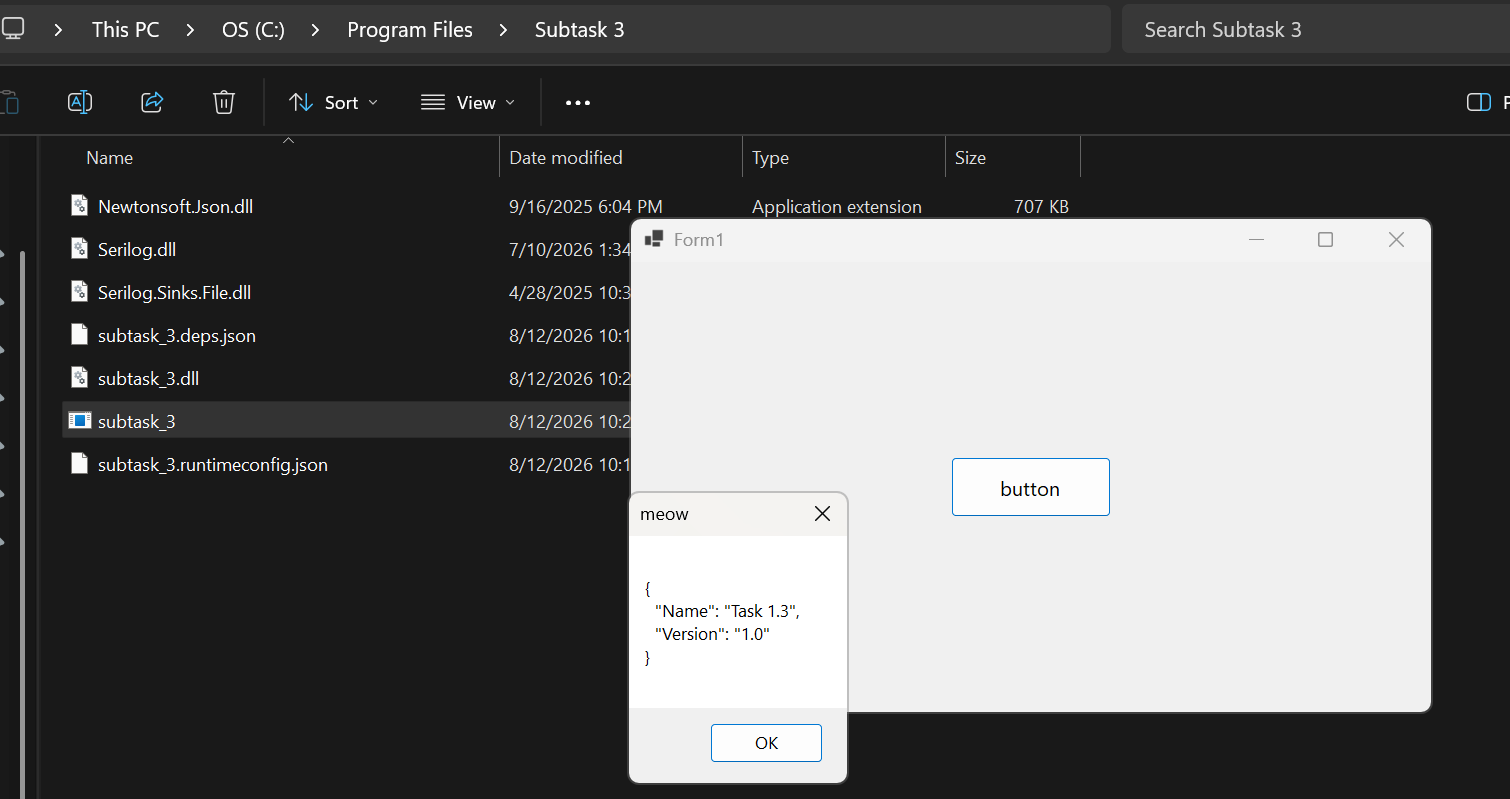
\includegraphics[scale=0.35]{images/3_run_app.jpg}
\vspace{-1em}
\caption{The application is installed using the MSI package and runs successfully.}
\end{figure}


% References
% \printbibliography
\end{document}